\chapter{On-shell techniques for tree-level amplitudes}
\label{ch:trees}
% use \chaptermark{}
% to alter or adjust the chapter heading in the running head


%\begin{svgraybox}
\abstract{
In this chapter we focus on the pole structure of tree-level amplitudes. We argue
that amplitudes factorise on these poles into lower-point amplitudes. Moreover, universal
factorisation structures emerge when two momenta become collinear as well as in the 
limit of low energy of a single particle---the soft limit. These factorisation properties
are the basis of an efficient technique for computing 
tree-level scattering amplitudes in gauge theories and gravity recursively---without
ever referring to Feynman rules or even a Lagrangian.
These recursion relations use as input lower-point amplitudes, so that 
the gauge redundancy, which is partly responsible for the complexity
of conventional Feynman graph calculations, is absent in this entirely on-shell based
formalism.
We then show the invariance of scattering amplitudes under Poincar\'e transformations, 
and introduce the conformal symmetry of gauge-theory tree-level amplitudes.
Finally, we highlight a surprising double-copy relation between gluon and graviton amplitudes.
}
%\end{svgraybox}


\section{Factorisation properties of tree-level amplitudes}
\label{sec:2.1}

Important insights and constraints on tree-level scattering amplitudes may be gained by thinking about them
as analytic functions of the external momenta. 
In this section we will restrict ourselves to the case of massless particles.
As we already argued in chapter \ref{ch:intro} with figure~\ref{Fig:regionmomenta}, 
tree-level amplitudes have simple poles in multi-particle channels. 
This can be seen from the Feynman diagrammatic expansion. Take all diagrams which have a propagator $\sim 1 / P_{ij}^2$, where  $P_{ij}=p_{i}+\ldots +p_{j}$ is a sum of external momenta (which will be adjacent for colour-ordered amplitudes, or an arbitrary subset in gravity).
We call $P_{ij}$ the \emph{region momentum}, as it is the total momentum associated to the
 region of momenta $\{p_{i},\ldots, p_{j}\}$. %
As $P_{ij}$ goes on shell, $P_{ij}^{2}\to 0$, these singular diagrams
will collect into a product of two on-shell amplitudes, to the left and right hand
sides of the divergent propagator, in a mechanism known as
\emph{factorisation}. This process is illustrated in
figure~\ref{fig:factorization}. We can understand the details of the procedure
by studying the Feynman rules for the propagator that goes on-shell directly, each of which has
the generic form
\be
\frac{\i \, N(P_{ij})}{P_{ij}^2} \,,
\ee
where the numerator $N(P_{ij})$ depends on the type of particle.
For example, for the specific case of gluons in the axial gauge ($n^\mu A_\mu=0$) 
we would have
$N(P)\to N_g^{\mu\nu}(P,n) = -\eta^{\mu\nu}+(P^\mu n^\nu+P^\nu
n^\mu)/(P\cdot n)$. In the limit $P_{ij}^{2}\to 0$ the numerator $N$ can be
rewritten in terms of the spin sum over external polarisation vectors or
wave-functions. Again for the case of gluons, following the results of exercise~\ref{Ex:1.7}, we have that
\be
N_g^{\mu\nu}(P,n) \overset{P^2\to 0}{\to} \sum_{h=\pm} \epsilon_{h}^{\mu}(P) \epsilon_{h}^{*\nu}(P) =  \sum_{h=\pm} \epsilon_{h}^{\mu}(P) \epsilon_{-h}^{\nu}(-P) \, .
\ee
The polarisation vectors combine with the Feynman diagram components on either
side of the divergent propagator to form on-shell amplitudes. A schematic form
for a general particle type can be written as
\be
\label{eq:multiparticlepole}
A_{n}^{\text{tree}}(1,\ldots, n) \stackrel{{}_{P_{ij}^{2}\to 0}}{\longrightarrow}  \sum_{s\in s_{\rm P}}
A_{L}^{\text{tree}}\bigl(i,i+1,\ldots,j, -P_{ij}^{\bar{s}}\bigr) \frac{n_{\rm P}}{P_{ij}^{2}} A_{R}^{\text{tree}}\bigl(P_{ij}^{s},j+1,\ldots, i-1\bigr) \, ,
\ee
where P indicates the particle type of the propagator with momentum $P_{ij}$,
$s_{\rm P}$ are its possible spin states and $n_{\rm P}$ is a particle-dependent constant.
As we see from the discussion above, for gluons $s_{\rm gluon} = \pm$ are the two
helicities and $n_{\rm gluon} = \i$, for spin-$\half$ fermions one can show that $s_{\rm fermion} =
\pm \nicehalf$ and $n_{\rm fermion} = 1$, while spin $0$ has $s_{\rm scalar} = 0$ and $n_{\rm scalar}=\i$. Other particle
types are simple to determine following the same argument. Factorisation will
also occur in the case of massive propagators where $P_{ij}^2\to m_{ij}^2$
where $m_{ij}$ is the mass of propagating particle.

%
\begin{figure}[t]
   \centering
  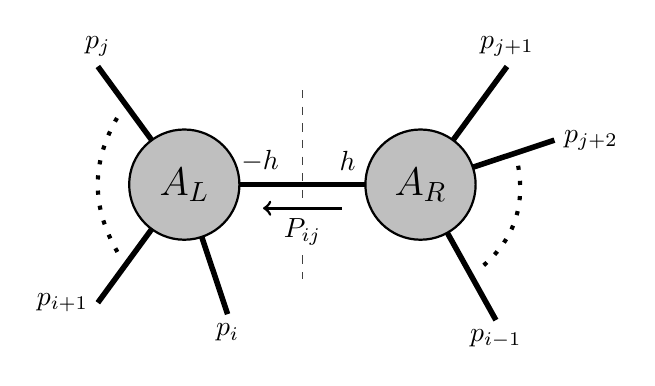
\begin{tikzpicture}[baseline={(current bounding box.center)}, scale =1.0]
  \coordinate (i) at (70:2);
  \coordinate (n-4) at (-30:2.3);
  \coordinate (n-3) at (-18:2.5);
  \coordinate (n-2) at (-5:2.6);
  \coordinate (i) at (30:3);
  \coordinate (i+1) at (10:3.25);
  \coordinate (n) at (-35:3);
  \coordinate (1) at (-120:1.9);
  \coordinate (2) at (-150:3);
  \coordinate (3) at (-170:2.5);
  \coordinate (4) at (-190:2.5);
  \coordinate (5) at (-180:2.5);
  \coordinate (i-1) at (-210:3);
  \coordinate (x) at (-1.5,0);
  \coordinate (y) at (1.5,0);
  \draw [dashed, line width=0.5pt, color = darkgray] (0,1.2) to (0,-0.2); 
  \draw [dashed, line width=0.5pt, color = darkgray] (0,-0.9) to (0,-1.2); 
  \draw [solid, line width=2pt] (y) to (x);
  \draw [->, line width=1pt] (0.5, -0.3) to (-0.5, -0.3);
  \draw (0,-0.6) node {$P_{ij}$};
%  \draw [solid,line width=2pt, {Latex[length=3mm]}-] (-0.3,0) to (0,0); 
  \draw [solid, line width=2pt] (x) -- (1);
  \draw [solid, line width=2pt] (x) -- (2);
  \draw [solid, line width=2pt] (y) -- (i+1); 
  \draw [solid, line width=2pt] (y) -- (n); 
  \draw [solid, line width=2pt] (y) -- (i); 
  \draw [solid, line width=2pt] (x) -- (i-1); 
  \draw [loosely dotted, line width=1.5pt] (-160:2.5) to[bend left=30] ((-200:2.5);;
  \draw [loosely dotted, line width=1.5pt] (5:2.75) to[bend left=30] (-25:2.5);
  \draw (1) node [below] {$p_{i}$};
  \draw (2) node [left] {$p_{i+1}$};
  \draw (n) node [below] {$p_{i-1}$};
  \draw (i+1) node [right] {$p_{j+2}$};
  \draw (i) node [above] {$p_{j+1}$};
  \draw (i-1) node [above] {$p_{j}$};
  \draw (-0.9,0.3) node [right] {$-h$};            
  \draw (0.8,0.3) node [left] {$h$};
  \draw [fill=lightgray,thick, draw=black] (x) circle (0.7);
  \draw [fill=lightgray,thick, draw=black] (y) circle (0.7);
  \draw (x) node {\Large $A_L$};
  \draw (y) node {\Large $A_R$};                       
\end{tikzpicture}
   \caption{The factorisation of a colour-ordered amplitude on the multi-particle
   pole $P_{ij}=p_{i}+p_{i+1} + \ldots + p_{j}$ when $P_{ij}^{2}\to 0$. Here $h$ denotes the
   helicity of the particles crossing the pole.}
   \label{fig:factorization}
\end{figure}

\subsection{Collinear limits}
\label{sect:collinear}

A special case of factorisation is the two-particle pole also known as \emph{collinear} singularity. Without loss of generality
we take the two collinear particles to be 1 and 2. 
We then have $(p_{1}+p_{2})^{2}=0$,
which implies $p_{1}\cdot p_{2}=0$ or \emph{collinearity} $p_{1}\parallel p_{2}$. We
again concentrate on the massless case.
In fact, since the factorisation now involves a three-particle amplitude, 
such a pole can only occur for collinear external momenta.
We already know from the discussion in the previous chapter that three-point amplitudes are subtle.
In the strict collinear limit $p_{1} \parallel p_{2}$ we may parametrise the collinear momenta $p_1$ and $p_2$ as
%
\be
p_{1}^{\mu}= x\, P^{\mu}\, ,  \qquad \qquad p_{2}^{\mu}= (1-x)\, P^{\mu} \,,
\ee
%
with the total collinear momentum $P=p_{1} + p_{2}$, and $x$ parametrising the amount of $P$ distribution over $p_{1}$
and $p_{2}$.
Tree-level amplitudes have a universal (singular) behaviour in the collinear limit governed by the
\emph{splitting functions},
\begin{align} \label{eq:collinear_limit}
A_{n}^{\rm tree}\bigl(1^{h_{1}}, 2^{h_{2}}, \ldots \bigr) 
\stackrel{1 \parallel 2}{\longrightarrow} \sum_{h= \pm} {\rm Split}^{\rm tree}_{h}\bigl(x,1^{h_{1}},2^{h_{2}}\bigr) \, A_{n-1}^{\rm tree}\bigl(P^{-h}, \ldots \bigr)\,,
\end{align}
as a special case of \eqn{eq:multiparticlepole}. In fact, the splitting functions are related to the three-particle amplitudes as
%
\be
\label{SplitfromFact}
 {\rm Split}^{\rm tree}_{h}\bigl(x,1^{h_{1}},2^{h_{2}}\bigr) = \lim_{P^2\to 0}\, A_{3}^{\text{tree}}\bigl(1^{h_{1}},2^{h_{2}},-P^{h}\bigr)\, \frac{\i}{P^{2}} \,.
\ee
%
The splitting functions depend on the helicities of the collinear gluons but are independent
of the helicities of the other legs $\{3,\ldots,n\}$ not participating in the collinear limit. This is
known as the universality of the splitting functions.
%
\begin{svgraybox}{\bf Gluon splitting functions.}
For collinear gluons the splitting functions are given by
\begin{align}
\label{splittingfunctions}
\begin{aligned}
&{\rm Split}_{+}^{\rm tree}(x, a^{+},b^{+}) = 0 \,,  &  
& {\rm Split}_{-}^{\rm tree}(x, a^{+},b^{+}) = \frac{g}{\sqrt{x (1-x)} \vev{a b}} \,, \\
&{\rm Split}_{+}^{\rm tree}(x, a^{+},b^{-}) = -\frac{(1-x)^2\, g}{\sqrt{x(1-x )} \vev{a b}} \,, 
& 
& {\rm Split}_{-}^{\rm tree}(x, a^{+},b^{-}) = - \frac{x^2\, g}{\sqrt{x (1-x)} [{a b}]}  \,.
\end{aligned} \end{align}
The remaining splitting functions may be obtained by parity
\begin{align}
\label{Splitparity}
{\rm Split}_{h}^{\rm tree}(x, a^{-\lambda_a},b^{-\lambda_b}) =   {\rm Split}_{-h}^{\rm tree}(x, a^{\lambda_a},b^{\lambda_b}) \Bigl|_{\vev{a b} \leftrightarrow [ba]} \,.
\end{align}
\end{svgraybox}
%
We shall now derive these expressions from our knowledge of the three-point MHV amplitude~\eqref{3pointmhv,3pointmhvbar}.
As the collinear kinematics is subtle, it is advantageous to systematically approach the collinear configuration as 
%
\bal{
& |1\rangle = \cos\phi\, |P\rangle -z\, \sin\phi\, |r\rangle \,, \qquad
& |1] = \cos\phi\, |P] -z\, \sin\phi\, |r] \,, \\
& |2\rangle = \sin\phi\, |P\rangle +z\, \cos\phi\, |r\rangle \,, \qquad
& |2] = \sin\phi\, |P] +z\, \cos\phi\, |r] \,
}
%
in the limit $z\to 0$.
Here $P^{\mu}=p_{1}^{\mu}+p_{2}^{\mu}+ \cO(z^{2})$ is the limiting collinear momentum vector,
and $r^{\mu}$ is a null reference momentum not parallel to $P^{\mu}$. Moreover, the collinear parameter above is $x=\cos^{2}\phi$. 
This parametrises the four-momenta of the collinear particles as
\bal{ \label{eq:momentadef}
p_{1}&= \cos^{2}\phi\, P - z\, \cos\phi\sin\phi\, \bigl(|P\rangle [r| + |r\rangle [P| \bigr) + z^{2} \, \sin^{2}\phi\,r \,,
\\
p_{2}&= \sin^{2}\phi\, P + z\, \cos\phi\sin\phi\, \bigl(|P\rangle [r| + |r\rangle [P| \bigr) + z^{2} \, \cos^{2}\phi\,r \,,
}
%
implying that $p_{1}+p_{2}=P+z^{2}\,r$, as claimed. One then has
%
\begin{align}
\vev{12} =& z \vev{Pr}\,,  \qquad  \vev{1P}=z \sin\phi\, \vev{Pr}\,, \qquad \vev{2P}=-z \cos\phi\, \vev{Pr}\,, \nn \\
 \bev{12} =& z \bev{Pr}\,,  \qquad  \bev{1P}=z \sin\phi\, \bev{Pr}\,, \qquad \bev{2P}=-z \cos\phi\, \bev{Pr} \, , \\
(p_{1}+p_{2})^{2}=&z^{2} \vev{Pr}\bev{rP} \,. \nn
\end{align}
%
The splitting functions~\eqref{splittingfunctions}
follow immediately from \eqn{SplitfromFact} and the two MHV three-point amplitudes~\eqref{3pointmhv,3pointmhvbar} upon using the above identities. 
The vanishing of ${\rm Split}_{+}^{\rm tree}(x,1^{+},2^{+})$
follows from the vanishing all-plus amplitude. Using the $\text{MHV}_{3}$ amplitude
of \eqn{3pointmhv}\footnote{Recall our convention~\eqref{negpspin} that $|-P\rangle= \i |P\rangle$ and  $|-P]= \i |P]$.} we find
%
\be
{\rm Split}_{-}^{\rm tree}(x,1^{+},2^{-}) =\frac{-\i g\vev{2(-P)}^{3}}{\vev{21}\,\vev{1(-P)}}\, \frac{\i}{(p_{1}+p_{2})^{2}}
= -\frac{\cos\phi^{3}g}{z\sin\phi \bev{Pr}} \,,
\ee
%
as well as using the $\widebar{\text{MHV}}_{3}$ amplitude of \eqn{3pointmhvbar},
%
\bal{
{\rm Split}_{-}^{\rm tree}(x,1^{+},2^{+}) &=  \frac{\i g[12]^{3}}{[1(-P)]\,[(-P)2]}\, \frac{\i}{(p_{1}+p_{2})^{2}}
%
= \frac{g}{z\cos\phi\sin\phi \vev{Pr}} \,, \\
{\rm Split}_{+}^{\rm tree}(x,1^{+},2^{-}) & =\frac{\i g[1(-P)]^{3}}{[12]\,[2(-P)]}\, \frac{\i}{(p_{1}+p_{2})^{2}}
%
= -\frac{\sin\phi^{3}g}{z\cos\phi \vev{Pr}}\, ,\nn
}
%
which prove the relations \eqref{splittingfunctions}. 

\newpage

\begin{example}{Example: Collinear limits of the five-point MHV amplitude} 
%
Let us use this result to test our conjectured five-point MHV amplitude~\eqref{ParkeTaylor1} from chapter \ref{ch:intro} for consistency under collinear limits. We set $g=1$ for convenience. We~have
\begin{align} \begin{aligned}
\i A_{5}^{\rm tree}(1^{-}, 2^{-}, 3^{+}, 4^{+}, 5^{+} ) & = \frac{ \vev{12}^4}{\vev{12}\vev{23}\vev{34}\vev{45}\vev{51}}  \\
& \stackrel{4 \parallel 5}{\longrightarrow} \frac{1}{\sqrt{x (1-x)} \vev{45}} \times \frac{ \vev{12}^4}{\vev{12}\vev{23}\vev{3 P} \vev{P 1}} \\
& = {\rm Split}_{-}^{\rm tree}(x, 4^{+}, 5^{+}) \times \i A_{4}^{\rm tree}(1^{-}, 2^{-}, 3^{+}, P^{+} ) \,,
\end{aligned} \end{align}
where we parametrised the collinear limit by
$|4\rangle= \sqrt{x} |P\rangle$ and $|5\rangle = \sqrt{1-x}|P\rangle$.
Indeed we find agreement with the second function in \eqn{splittingfunctions}.
Next, we take the collinear limit in a $(-+)$ channel.
We have
\begin{align} \begin{aligned}
\i A_{5}^{\rm tree}(1^{-}, 2^{-}, 3^{+}, 4^{+}, 5^{+} ) & \stackrel{2 \parallel 3}{\longrightarrow} \frac{x^2}{\sqrt{x (1-x)}} \frac{1}{\vev{23}} \frac{ \vev{1P}^4}{\vev{1 P}\vev{P 4}\vev{45}\vev{51}}  \\
& = {\rm Split}_{+}^{\rm tree}(z,2^{-},3^{+}) \times \i A_{4}^{\rm tree}(1^{-}, P^{-}, 4^{+}, 5^{+}) \,,
\end{aligned} \end{align}
from which we deduce \be{\rm Split}_{+}^{\rm tree}(x,a^{-},b^{+})= \frac{x^{2}}{\sqrt{x(1-x)}\,\vev{ab}}\,,
\ee 
in agreement with the third expression in \eqn{splittingfunctions} whilst swapping $a$ and $b$ (and $x\to 1-x$).
In order to check the fourth function we consider the collinear limit in a $(+-)$-channel,
%
\be
A_{5}^{\rm tree}(1^{-}, 2^{-}, 3^{+}, 4^{+}, 5^{+} )\stackrel{5 \parallel 1}{\longrightarrow}
\underbrace{\frac{(1-x)^{2}}{\sqrt{x(1-x)}\, \vev{51}}}_{{\rm Split}_{+}^{\rm tree}(x,5^{+},1^{-})}\,  A_{4}^{\rm tree}(P^{-}, 2^{-}, 3^{+}, 4^{+} ) \,,
\ee
%
yielding the desired result via parity~\eqref{Splitparity}. In order to check the vanishing of the uniform
helicity splitting function in \eqn{splittingfunctions} we 
have to study the collinear factorisation of the 6-point MHV amplitude with the helicity
distributions
$A_{6}^{\rm tree}(1^{-}, 2^{-}, 3^{+}, 4^{+}, 5^{+},6^{+} )$ along the legs 5 and 6.
\end{example}

\newpage

\begin{exer}{The vanishing splitting function ${\rm Split}_{+}^{\rm tree}(x, a^{+},b^{+})$}
\label{Exer:2.1}
Show that ${\rm Split}_{+}^{\rm tree}(x, a^{+},b^{+}) = 0$ by studying the factorisation properties of the six-gluon MHV tree amplitude $A_{6}^{\rm tree}(1^{-}, 2^{-}, 3^{+}, 4^{+}, 5^{+}, 6^{+} )$ from \eqn{ParkeTaylor1} in the collinear limit $5 \parallel 6$. 
For the solution see \hyperref[Sol:2.1]{chapter~5}.
\end{exer}

\begin{svgraybox}{\bf Absence of multi-particle poles in MHV amplitudes.}
General $n$-gluon scattering amplitudes have multi-particle poles when region momenta 
go on-shell. However, MHV tree-amplitudes are special, and in fact \emph{only}
 have two-particle poles or collinear singularities. 
The reason is the following. 
Consider the general factorisation formula~\eqref{eq:multiparticlepole}.
In a factorisation of an MHV amplitude there
are only three negative-helicity legs (corresponding to the two external negative helicities, and one for the internal
on-shell propagator) that are distributed over two partial amplitudes. 
However, we saw in the previous chapter that  $A_{n}(1^{\pm},2^{+},\ldots, n^{+}) = 0$ (for $n > 3$).
Therefore, either $A_{L}$ or $A_{R}$ in \eqn{eq:multiparticlepole} is always zero unless one 
partial amplitude is a three-particle amplitude. The latter case corresponds to a two-particle pole or collinear
singularity, as discussed above.
\end{svgraybox}

\subsection{Soft theorems}

We continue our quest in the factorisations of scattering amplitudes with a kinematical limit
subject to just a \emph{single} leg: the soft limit. Here one particle involved in the scattering process 
has a very low energy---it is soft. Specifically, it refers to the limit where the four-momentum of the particle 
goes to zero. Again the tree-amplitude displays a universal factorisation property 
for photon, gluon and graviton amplitudes into a lower-point amplitude and a soft function. 
In order to take the limit, we parametrise the soft momentum of leg $s$ as
$p_{s}^{\mu} =  \delta\,  q^{\mu}$ and take $ \delta\, \to 0$ (do not confuse $ \delta\,  q^{\mu}$ 
with a variation). The soft theorems state that
%
\be
\label{centralsoft}
A_{n+1}^{\text{tree}} ( \delta\,  q, 1,\ldots , n) \stackrel{ \delta\,\to 0}{\longrightarrow}
S[ \delta\,   q,  \{p_1,\ldots,p_{n}\}]\, A_{n}^{\text{tree}}(1,\ldots , n)\, ,
\ee
%
which is illustrated in figure~\ref{fig:softthm}. 
%
\begin{figure}[t]
   $$
  \begin{tikzpicture}[baseline={(current bounding box.center)}, scale = 0.9]
 \coordinate (q) at (0:2);
\coordinate (1) at (-55:2);
\coordinate (2) at (-125:2);
\coordinate (3) at (125:2);
\coordinate (n) at (55:2);
\coordinate (0) at (0,0);
\draw [solid,line width=1pt] (0) -- (1);
\draw [solid, line width=1pt] (0) -- (2);
\draw [solid, line width=1pt] (0) -- (3); 
\draw [solid,line width=1pt] (0) -- (n); 
\draw [graviton] (0) -- (q); 
\draw [loosely dotted, line width=1.5pt] (-135:1.2) to[bend left=70] (135:1.2);

  \draw (1) node [below] {$p_{1}$};
  \draw (2) node [left] {$p_{2}$};
    \draw (3) node [left] {$p_{n-1}$};
  \draw (n) node [right] {$p_{n}$};
    \draw (q) node [right] {$\mathbf{ \delta\,}\, q$};
    \draw [fill=lightgray,thick, draw=black] (0) circle (0.7);
 \draw (0) node {\Large $A_{n+1}$};                       
 \end{tikzpicture}
 \stackrel{\delta\to 0}{\longrightarrow}
  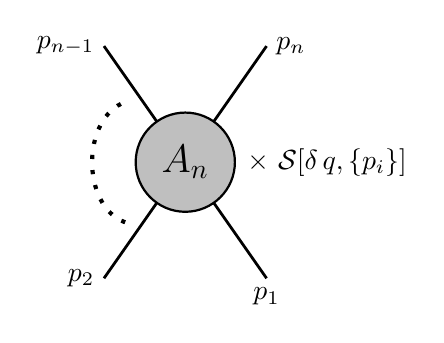
\begin{tikzpicture}[baseline={(current bounding box.center)}, scale = 0.9]
% \coordinate (q) at (0:2);
\coordinate (1) at (-55:2);
\coordinate (2) at (-125:2);
\coordinate (3) at (125:2);
\coordinate (n) at (55:2);
\coordinate (0) at (0,0);
\coordinate (here) at (2,0);
\draw [solid,line width=1pt] (0) -- (1);
\draw [solid, line width=1pt] (0) -- (2);
\draw [solid, line width=1pt] (0) -- (3); 
\draw [solid,line width=1pt] (0) -- (n); 
%\draw [graviton,  -{Latex[length=3mm]}] (0) -- (q); 
\draw [loosely dotted, line width=1.5pt] (-135:1.2) to[bend left=70] (135:1.2);

  \draw (1) node [below] {$p_{1}$};
  \draw (2) node [left] {$p_{2}$};
    \draw (3) node [left] {$p_{n-1}$};
  \draw (n) node [right] {$p_{n}$};
 %   \draw (q) node [right] {$\mathbf{\delta}\, q$};
    \draw [fill=lightgray,thick, draw=black] (0) circle (0.7);
 \draw (0) node {\Large $A_{n}$};      
 \draw  (here) node {$\times\,  \, \mathcal{S}[ \delta\, q, \{p_{i}\} ]$};                 
 \end{tikzpicture}
  $$
   \caption{The soft factorisation of a generic $(n+1)$-particle amplitude. The soft function $\mathcal{S}[ \delta\, q, \{p_{i}\} ]$
   only depends on the momenta (not the polarisations) of the hard legs.}
   \label{fig:softthm}
\end{figure}
%
%
The factorised soft function $S[ \delta\,   q,  \{p_1,\ldots,p_{n}\}]$
 depends on the momentum $ \delta\, \, q$ and helicity of the soft particle, as well as the
momenta of the remaining hard legs $\{p_{a}\}$. It is however independent  of 
the helicities and even particle types of the remaining hard legs, which may be massless or massive. 
The soft function diverges as $1/\delta$ at leading order, and also contains universal sub-leading~pieces:
\be
\label{softtheoremgeneral}
 S[ \delta\,   q, \{p_{a}\}] = \frac{1}{\delta} \mathcal{S}^{[0]}(q) + \mathcal{S}^{[1]}(q)
 + \delta\, \mathcal{S}^{[2]}(q)  + \cO\bigl(\delta^{2}\bigr)\,.
 \ee
 It takes a universal form for photons~\cite{ch2_Low:1958sn}, gluons and gravity~\cite{ch2_Weinberg:1964ew}, remarkably not only
 to leading order, but also to sub-leading order $\mathcal{S}^{[1]}(q)$ for gauge theories, and even to
sub-sub-leading order $\mathcal{S}^{[2]}(q)$ for gravity~\cite{ch2_Cachazo:2014fwa}. 

\begin{svgraybox}{\bf Leading soft theorems.}
The leading soft divergences take the universal form 
%
\begin{equation}
 \frac{1}{\delta} \mathcal{S}^{[0]}(\delta  q)= \begin{cases} 
  \displaystyle \frac{1}{\delta} {\cal S}^{[0]}_\text{EM} = \frac{1}{\delta} \,
    \sum_{a=1}^{n} e_{a}\frac{\epsilon\cdot p_{a}}{p_{a}\cdot q} \,, & \text{photon, }\\[12pt]  

  \displaystyle \frac{1}{\delta} {\cal S}^{[0]}_\text{YM} = \frac{g}{\delta\sqrt{2}} \,
    \bigg(\frac{\epsilon\cdot p_{1}}{p_{1}\cdot q}-\frac{\epsilon\cdot p_{n}}{p_{n}\cdot q}\bigg)\,, & \text{colour-ordered gluon, }\\[12pt]  
    \displaystyle \frac{1}{\delta} {\cal S}^{[0]}_\text{GR} = \frac{\kappa}{\delta} \, 
    \sum_{a=1}^{n}  \frac{\epsilon_{\mu\nu}\, p_{a}^{\mu}\, p_{a}^{\nu}}{p_{a} \cdot q} \,,
    &\text{graviton. } \end{cases}
  \label{eq:S0explicit}
\end{equation}
%
Here $\epsilon$ denotes the polarisation vector (tensor) of the soft particle,  $e_{a}$ denotes the $\text{U}(1)$  (electromagnetic) charge of the hard particle~$a$. 
\end{svgraybox}
%
These results can be made plausible through the following argument based on Feynman diagrams. For a tree-level amplitude the soft leg $\delta \, q$ is attached
either via a three-point coupling to an outgoing hard leg $a$, or to the ``bulk'' of the remaining~amplitude:
%
\be
\raisebox{0.6cm}{$A_{n}^{\text{tree}}(\delta\, q, \{p_{a}\})=$} 
 \begin{tikzpicture}[baseline={(current bounding box.center)}]
 \coordinate (0) at (-1,0);
\coordinate (b) at (0.25,0);
\coordinate (a) at (45:1);
\coordinate (q) at (-45:1);
\coordinate (n) at (145:1.6);
\coordinate (1) at (-145:1.6);
\coordinate (expl) at (0,-1.7);
\coordinate (mid) at (-0.2,-0.1);
\draw [solid,line width=1pt] (0) -- (1);
\draw [solid, line width=1pt] (0) -- (n);
\draw [solid, line width=1pt] (0) -- (b);
\draw [solid, line width=1pt] (b) -- (a);
\draw [graviton,] (b) -- (q); 
\draw [loosely dotted, line width=1.5pt] (-160:1.5) to[bend left=70] (160:1.5);
 \draw [fill=lightgray,thick, draw=black] (0) circle (0.4);
  \draw [fill] (b) circle (.08);
   \draw (a) node [right] {$a$};
      \draw (q) node [right] {$\delta \, q$};
      \draw [dashed, ->] (expl) to [bend left=10]  (mid);
        \draw (expl) node [right] {$\displaystyle \frac{1}{(p_{a}+\delta \,q)^{2}-m_{a}^{2}}\stackrel{\delta\to 0}{=}
        \frac{1}{2\delta} \frac{1}{p_{a}\cdot q}$};
%\end{tikzpicture}
\draw (1.5,0) node [right] {$+$} ;
\draw (-2.75,0) node [right] {$\displaystyle \sum_{a=1}^{n}$} ;
%%+ \quad 
%begin{tikzpicture}[baseline={(current bounding box.center)}]
 \coordinate (0p) at (-1,0);
%\coordinate (b) at (0,0);
\coordinate (ap) at (90:.5);
\coordinate (qp) at (-90:.5);
\coordinate (np) at (145:1.6);
\coordinate (1p) at (-145:1.6);
\begin{scope}[every coordinate/.style={shift={(4,0)}}]
\draw [solid,line width=1pt] ([c] 0p) -- ([c] 1p);
\draw [solid, line width=1pt] ([c] 0p) -- ([c] np);
%\draw [solid, line width=1pt] (0) -- (b);
\draw [solid, line width=1pt] ([c] 0p) -- ([c] ap);
\draw [graviton] ([c] 0p) -- ([c] qp); 
\draw [loosely dotted, line width=1.5pt] ([c] -160:1.5) to[bend left=70] ([c] 160:1.5);
 \draw [fill=lightgray,thick, draw=black] ([c] 0p) circle (0.4);
  \draw ([c] ap) node [right] {$a$};
      \draw ([c] qp) node [right] {$\delta \, q$}; 
%  \draw [fill] (b) circle (.08);
\end{scope}
\end{tikzpicture}
\ee
%
We see that the divergence of the leading order soft function 
solely arises from the three-point coupling of the gauge or graviton field
to the hard leg $a$. In the case of an amplitude with $n$-scalars and a soft photon or graviton these couplings
take the form
%
\be
\begin{tikzpicture}[baseline={(current bounding box.center)}]
 \coordinate (0) at (-1,0);
\coordinate (b) at (0.25,0);
\coordinate (a) at (45:1);
\coordinate (q) at (-45:1);
\draw [solid,line width=1pt] (0) -- (b);
\draw [solid, line width=1pt] (b) -- (a);
\draw [graviton,] (b) -- (q); 
  \draw [fill] (b) circle (.08);
   \draw (a) node [right] {$a$};
      \draw (q) node [right] {$\delta \, q$};
\end{tikzpicture}  
\propto  \quad
\begin{cases} 
  \displaystyle  e_{a}\, \epsilon\cdot p_{a} \,,  & \text{photon, }\\[12pt]  
    \displaystyle \kappa \,\epsilon_{\mu\nu}\, p_{a}^{\mu}\, p_{a}^{\nu} \,,
    &\text{graviton, } \end{cases}
\ee
which fixes the soft functions in \eqn{eq:S0explicit} up to an overall factor. In the case of a colour-ordered
pure gluon amplitude with one soft gluon leg, $A_{n}^{\text{tree}}(1,\ldots,n,\delta \, q)$, the soft leg can couple
either  to the hard gluon leg $1$ or $n$ due to colour ordering.
A detailed look at the Feynman rules~\eqref{Feynrulveert} then reveals the coupling $\pm g\, p_{a}\cdot\epsilon$ with
$a=1,n$ at leading order in $\delta$ with a relative sign factor reproducing the form of~\eqn{eq:S0explicit}.

It is instructive to study the gauge invariance of the leading soft functions~\eqref{eq:S0explicit}. Gauge
invariance requires the full amplitude $A_{n+1}(\delta \, q, p_{1},\ldots , p_{n})$ to vanish under the
transformation $\epsilon^{\mu}\to q^{\mu}$ (in the graviton case we again take 
$\epsilon_{\mu\nu}=\epsilon_\mu\epsilon_{\nu}$). Hence, by consistency, the soft functions in \eqn{eq:S0explicit}  
need to vanish:
%
\begin{equation}
  \mathcal{S}^{[0]}(\delta \, q)\Bigr |_{\epsilon\to q}= \begin{cases} 
  \displaystyle \quad \,
    \sum_{a=1}^{n} e_{a}=0 \,, & \text{photon, }\\[12pt]  
  \displaystyle  \,\,\, \frac{g}{\sqrt{2}} (1-1)=0 \,, & \text{gluon, } \\[12pt]  
    \displaystyle \kappa \, q_{\mu}
    \sum_{a=1}^{n}   p_{a}^{\mu}=0  \,,
    &\text{graviton. } \end{cases}
\end{equation}
%
They indeed vanish due to total charge conservation in the electromagnetic or total momentum conservation
in the gravitational case (provided the gravitational coupling is universal to all matter). Hence these soft theorems
are intimately connected to fundamental symmetries of space-time-matter.

\subsection{Spinor-helicity formulation of soft theorems}
It is instructive to translate the leading soft theorems to spinor-helicity language for the colour-ordered gluon
and graviton cases. The leading order soft factorisation states~that
\begin{align}
A_{n}^{\text{tree}}(\ldots, a, \delta q^{\pm}, b,\ldots) \stackrel{\delta\to 0}{\longrightarrow}
  \mathcal{S}^{[0]}(a,q^{\pm},b)\, A_{n-1}^{\text{tree}}(\ldots, a,  b,\ldots) \, .
\label{cosoftfactorization}
\end{align}
The factorised soft function depends on the momenta and helicities of the soft gluon and the
momenta of the colour-ordered neighbours $a$ and $b$. It is independent, however,  of 
the helicities and particle types of the neighbouring legs.
From considering the soft limit of an MHV amplitude one easily establishes that
%
\be
 \mathcal{S}_{\text{YM}}^{[0]}(a,q^{+},b) = g\frac{\vev{ab}}{\vev{aq}\vev{qb}} \, .
\ee
%
Via parity, in analogy to \eqn{Splitparity}, we find
%
\be \label{eq:SoftYM_minus}
\mathcal{S}_{\text{YM}}^{[0]}(a,q^{-},b) = -g\frac{\bev{ab}}{\bev{aq}\bev{qb}} \, .
\ee
%
Both results directly follow from \eqn{eq:S0explicit} as well. In the graviton case we deduce
%
\be
\mathcal{S}_{\text{GR}}^{[0]}(q^{++},1,\ldots, n) = \kappa \sum_{a=1}^{n}
\frac{\vev{xa}\vev{ya}\bev{qa}}{\vev{xq}\vev{yq}\vev{aq}}\, ,
\ee
%
where $x$ and $y$ are arbitrary reference spinors associated to the polarisation vectors of the soft~leg.


\begin{exer}{Soft functions in the spinor-helicity formalism}
\label{Ex:2.2}
Starting from eq.~\eqref{eq:S0explicit}, derive the leading soft functions for a colour-ordered gluon and a graviton in the spinor-helicity formalism.
For the solution see \hyperref[Sol:2.2]{chapter~5}.
\end{exer}


\subsection{Subleading soft theorems}
Remarkably, the universal soft factorisation survives to subleading order ($\cO\bigl(\delta^{0}\bigr)$) in the gauge theory, and even
sub-sub-leading order ($\cO\bigl(\delta\bigr)$) in the gravitational case, 
cf.~\eqn{softtheoremgeneral}. Here we just state the results. They may again
be derived from a careful study of gauge invariance and consistency arguments~\cite{ch2_Broedel:2014fsa,ch2_Bern:2014vva}.
The novelty is that the sub-leading soft functions are (necessarily) no longer true functions but rather  \emph{differential operators} in the external kinematical data. These then
act on the factorised hard scattering-amplitude.
Explicitly, one has the following sub-leading soft operator for a soft photon $q^{\mu}$ with polarisation 
$\epsilon^{\mu}$,
%
\be
\mathcal{S}_{\text{EM}}^{[1]}(q) = \sum_{a=1}^{n} e_{a} \frac{\epsilon_{\mu} q_{\nu}\, J_{a}^{\mu\nu}}{p_{a}\cdot q} \,,
\ee
%
with the local angular momentum operator
\be
J_{a}^{\mu\nu} = 2\, p_{a}^{[\mu} \frac{\partial}{\partial p_{a,\, \nu]}} 
+2\, \epsilon_{a}^{[\mu} \frac{\partial}{\partial \epsilon_{a,\, \nu]}} \, .
\ee
In the above $[\mu\nu]$ denotes anti-symmetrisation with unit weight, see Appendix \ref{sec:Conventions}.
Similarly, for a colour-ordered soft gluon we have
%
\be
\mathcal{S}_{\text{YM}}^{[1]}(n,q,1) = -\i \frac{g}{\sqrt{2}} \left (\frac{\epsilon_{\mu} q_{\nu}\, J_{1}^{\mu\nu}}{p_{1}\cdot q}
- \frac{\epsilon_{\mu} q_{\nu}\, J_{n}^{\mu\nu}}{p_{n}\cdot q} \right )\,,
\ee
%
while for a soft gravitons we have a sub-leading and sub-sub-leading soft operators of the forms
%
\bal{
\label{softnnGR}
\mathcal{S}_{\text{GR}}^{[1]}(q) &= -\i \kappa \sum_{a=1}^{n} \frac{\epsilon\cdot p_{a}\, \epsilon_{\mu} q_{\nu}\, J_{a}^{\mu\nu}}{p_{a}\cdot q} \,, \qquad 
\mathcal{S}_{\text{GR}}^{[2]}(q) = -\frac{\kappa}{2} \sum_{a=1}^{n} \frac{\bigl(\epsilon_{\mu} q_{\nu}\, J_{a}^{\mu\nu}\bigr)^{2}}{p_{a}\cdot q} \,.
}
%
Again, one may show that these sub-leading soft operators are consistent with gauge invariance. While this is trivial for
the gauge-theory operators by virtue of the anti-symmetry of $J^{\mu\nu}$, the gauge invariance of the gravitational $\mathcal{S}_{\text{EM}}^{[1]}(q)$ leads us to total
angular momentum conservation, 
%
\be
\mathcal{S}_{\text{GR}}^{[1]}(q)\Bigr |_{\epsilon\to q} = -\i \kappa \, \epsilon_{\mu} q_{\nu}\, 
\sum_{a=1}^{n} J_{a}^{\mu\nu} =0 \,,
\ee
%
nicely teaming up with the total momentum conservation in the leading case. Hence, the
gravitational soft theorems are directly connected to the Poincar\'e invariance of scattering amplitudes.

Expressed in spinor-helicity variables the sub-leading soft operators take the form
%
\bal{
\label{spinsubleadingsoft}
\mathcal{S}_{\text{YM}}^{[1]}(n,q^{+},1) &= g\left( \frac{\bev{q\partial_{n}}}{\vev{qn}}-
 \frac{\bev{q\partial_{1}}}{\vev{q1}} \right) \,, \\
 \mathcal{S}_{\text{GR}}^{[1]}(q^{+},1,\ldots, n) &= \frac{\kappa}{2}
 \sum_{a=1}^{n} \frac{\bev{aq}}{\vev{aq}}\left (\frac{\vev{ax}}{\vev{qx}} + 
  \frac{\vev{ay}}{\vev{qy}}\right)\, \bev{q\partial_{a}} \,,
  }
%
where as before $x$ and $y$ are arbitrary reference spinors. The sub-sub-leading gravity
operator of \eqn{softnnGR} in spinor-helicity variables simply reads
%
\be
 \mathcal{S}_{\text{GR}}^{[2]}(q^{+},1,\ldots, n) = \frac{\kappa}{2}
 \sum_{a=1}^{n} \frac{\bev{aq}}{\vev{aq}} \bev{q\partial_{a}}^{2}  \,,
\ee
%
and was found in~\cite{ch2_Cachazo:2014fwa}. 

An important subtlety for the sub-leading soft
theorems lies in balancing the total momentum conservation of the $(n+1)$-leg amplitude
with the soft leg and the factorised $n$-point hard amplitude. The
soft factorisation~\eqref{centralsoft} is really a distributional identity involving
delta-functions:
%
\begin{align}\begin{aligned}
\delta^{(D)}(\delta \, q + P) \, \mathcal{A}_{n+1}^{\text{tree}} (\delta \, q,\{p_{a}\}) \stackrel{\delta\to 0}{\longrightarrow}& \\
S[\delta \,  q,  \{p_{a}\}]\, & \delta^{(D)}(P)\,  \mathcal{A}_{n}^{\text{tree}}(1,\ldots , n)+ \cO\bigl(\delta^{j}\bigr)\, ,
\end{aligned}\end{align}
%
with $P=p_{1}+\ldots + p_{n}$ and $j=1$ or $2$ for gauge theory or gravity, respectively. This
in fact implies~that
%
\be
S[\delta \,  q,  \{p_{a}\}]\,  \delta^{(D)}(P) = \delta^{(D)}(\delta \, q + P)\, 
S[\delta \,  q,  \{p_{a}\}]\, ,
\ee
%
from which one may strongly constrain the $\delta$ expansion  of the soft
function $S[\delta \,  q,  \{p_{a}\}]$ using \eqn{softtheoremgeneral}.
It necessitates the sub-leading terms to be differential operators, and
even the functional forms of \eqn{spinsubleadingsoft} are fixed by the knowledge of the leading soft functions~\cite{ch2_Broedel:2014fsa}.


\begin{exer}{A $\bar{q}qggg$ amplitude from collinear and soft limits}
\label{Ex:qqggg}
In chapter~\ref{ch:intro} we established the following colour-ordered $\bar{q}qgg$ amplitudes involving a massless quark and anti-quark using colour-ordered Feynman rules:
\begin{align} \label{eq:Aqqgg1}
& A_{\bar q q  gg}^{\text{tree}}(1^{-}_{\bar q}, 2^{+}_{q}, 3^{+},4^{+}) = 0 \,, \\
 \label{eq:Aqqgg2}
& A_{\bar q q  gg}^{\text{tree}}(1^{-}_{\bar q}, 2^{+}_{q}, 3^{-},4^{+}) = -\i g^{2}
\frac{\vev{13}^{3}\, \vev{23}}
{\vev{12}\,\vev{23}\,\vev{34}\, \vev{41}}\, .
\end{align}
Use these and the discussed splitting and soft factorisation properties for gluonic legs to make a guess for the five-point single quark-line tree amplitude $A^{\text{tree}}_{\bar{q}qggg}(1^{-}_{\bar{q}}, 2^+_q, 3^-, 4^+, 5^+)$. Check your guess against all known factorisation properties.
%
Can you generalise your guess to the $n$-particle partial amplitudes \break $A^{\text{tree}}_{\bar{q}qg\ldots g}(1^{-}_{\bar{q}}, 2^+_q, 3^+, \ldots, n^+)$ and 
$A^{\text{tree}}_{\bar{q}qg\ldots g}(1^{-}_{\bar{q}}, 2^+_q, 3^-, 4^+, \ldots, n^+)$?
For the solution see \hyperref[Sol:qqggg]{chapter~5}.
\end{exer}



\section{BCFW recursion for gluon amplitudes}
\label{sec:2.2}

The Britto-Cachazo-Feng-Witten (BCFW) recursion relation~\cite{ch2_Britto:2004ap,ch2_Britto:2005fq} 
is an efficient way
to compute higher-point tree-level amplitudes
from lower-point ones. It does not make use of Feynman rules but builds upon
unitarity by artfully exploiting the
factorisation property of scattering amplitudes~\eqref{eq:multiparticlepole}
when region momenta go on-shell.
As we will see, our knowledge of the gluon (and graviton) three-point amplitudes 
of eqs.~\eqref{3pointmhv} and~\eqref{3pointmhvbar} allows for the construction of {\it all} higher-point tree-level amplitudes in a recursive fashion.
To begin with, let us concentrate on the colour-ordered case and leave the discussion of
gravitons for later. 
The central idea of the recursion is to consider a deformation 
in a {\it  single} complex variable $z$ of two adjacent momenta in a colour-ordered
 amplitude that maps
the  singularities of the amplitude into poles in  $z \in {\mathbb{C}}$.
For the tree-level $n$-gluon amplitude $A_{n}( p_{1}, \ldots p_{n})$ we introduce
the following complex shift of the helicity spinors
of two arbitrary adjacent particles, taken to be $1$ and $n$ without loss of generality:
\begin{align} \label{bcfw-n1}
\begin{split}
&\lambda_1 \rightarrow \hat{\lambda}_{1}(z) = \lambda_{1} - z \lambda_{n} \,, \qquad  \tla_{1}\rightarrow
\tla_{1} \, ,  \\
&\la_{n}\rightarrow
\la_{n} \, , \qquad\qquad \qquad \qquad 
\tilde{\lambda}_n \rightarrow \hat{\tilde\lambda}_{n}(z) = \tilde{\lambda}_{n} + z \tilde{\lambda}_{1} \, . 
\end{split}
\end{align}
We denote the shifted, $z$-dependent quantities by a hat.
This shift is often termed an $[n\, 1\ran$ shift.
It results in a  deformation of the  momenta, 
\begin{align}
\label{complexmamienta}
p_{1}^{\dot\alpha {\alpha}} \to \hat{p}_{1}^{\dot\alpha {\alpha}} (z) = 
\tilde{\lambda}_{1}^{\dot\alpha}\, (\lambda_{1} -z \lambda_{n})^{\alpha}  \,,\qquad
p_{n}^{\dot\alpha {\alpha}} \to \hat{p}_{n}^{\dot\alpha {\alpha}} (z) = (\tilde{\lambda}_{n} + z  \tilde{\lambda}_{1} )^{\dot\alpha}\, \lambda_{n}^{\alpha}  \,.
\end{align}
Importantly, the shift preserves both overall
 momentum conservation and the on-shell conditions:
\begin{equation}
\label{preservedpids}
\hat{p}_{1}(z) + \hat{p}_{n}(z) = p_{1} + p_{n}\, , \qquad 
\hat{p}_{1}^2(z) = 0\,,\qquad \hat{p}_{n}^{2}(z) = 0\, . 
\end{equation}
The $[n\, 1\ran$  shift generates
 a  one-parameter family of amplitudes,
 \be
 A_n(z) \coloneqq A_n \big(\hat{p}_1 (z), p_2, \ldots, p_{n-1}, \hat{p}_n(z)\big)\, .
 \ee 
Note that $\hat{p}_1$ and $\hat{p}_n$ in \eqn{complexmamienta} are now complex, 
as the underlying helicity spinors $\la_{1,n}$ and $\tla_{1,n}$ are
no-longer complex conjugates of each other.  This  makes  the three-point amplitudes 
involving these states of eqs.~\eqref{3pointmhv,3pointmhvbar}  non-vanishing. They will become the seeds of the recursion relation. 
%
What are the analytic properties of  the deformed amplitude $A_{n}(z)$?
Factorisation implies   that the deformed amplitude $A_{n}(z)$  has precisely
$n{-}3$ \emph{simple} poles in $z$. Using the region momenta  $P_{i}\coloneqq\sum_{j=1}^{i-1}p_{j}$, these $n{-}3$ poles take the form 
\begin{align}
\label{poleargumentbcfw}
\begin{split}
\frac{\i}{\hat{P}_{i}^2(z)} &
\coloneqq 
\frac{\i}{P_{i}^2 - z \, \langle n | P_{i} | 1 \rbrack} = -\frac{1}{\langle n | P_{i} | 1 \rbrack} 
\frac{\i}{z - z_{P_{i}} }
\, , 
\end{split}
\end{align}
where $\hat{P}_{i}(z) = \hat{p}_{1}(z) + p_{2} + \cdots p_{i-1}$, and 
%
\be
\label{zPidef}
z_{P_{i}}=\frac{P_{i}^{2}}{\lan n|P_{i}|1]}\, , \qquad \quad \forall i\in \{3,
\ldots ,n-1\}\, .
\ee
%
\begin{figure}[tt]
%%\fl
\begin{center}
\begin{equation*}
  \begin{tikzpicture}[baseline={(current bounding box.center)}, scale = 0.8]
  \tikzstyle{blob}=[
    circle,
    minimum size =1.5cm,
    draw=black,
    thick,
    fill=lightgray,
    text=black
]
\begin{feynman}
\coordinate (i) at (70:2);
\coordinate (n-1) at (-30:2);
\coordinate (n) at (-70:2);
\coordinate (1) at (-110:2);
\coordinate (2) at (-150:2);
\coordinate (3) at (-190:2);
\coordinate (i-1) at (-250:2);
\coordinate (x) at (0,0);
\draw [gluon] (x) -- (1);
\draw [gluon] (x) -- (2);
\draw [gluon] (x) -- (3); 
\draw [gluon] (x) -- (n-1); 
\draw [gluon] (x) -- (n); 
\draw [gluon] (x) -- (i); 
\draw [gluon] (x) -- (i-1); 
  \draw (1) node [below] {$\hat{1}(z)$};
  \draw (2) node [left] {$2$};
  \draw (3) node [left] {$3$};
  \draw (n) node [below] {$\hat{n}(z)$};
    \draw (n-1) node [right] {$n-1$};
        \draw (i) node [above] {$i$};
            \draw (i-1) node [above] {$i-1$};
   \draw [loosely dotted, line width=1.5pt] (-200:1.2) to[bend left=40] (-240:1.2);         
   \draw [loosely dotted, line width=1.5pt] (60:1.2) to[bend left=50] (-20:1.2); 
   \draw [fill=lightgray,thick, draw=black] (x) circle (0.7);
 \draw (x) node {$A_{n}(z)$};    
%
\draw (1.5,0) node [right] {$\displaystyle 
{\buildrel z\to z_{P_i} \over
{\relbar\mskip-1mu\joinrel\rightarrow}}
\frac{1}{z-z_{Pi}}\, \sum_h $};
\coordinate (ip) at (30:3);
\coordinate (i+1p) at (10:3.25);
\coordinate (np) at (-55:2.1);
\coordinate (1p) at (-120:1.9);
\coordinate (2p) at (-150:3);
\coordinate (i-1p) at (-210:3);
\coordinate (xp) at (-1.5,0);
\coordinate (yp) at (1.5,0);
\begin{scope}[every coordinate/.style={shift={(7.5,0)}}]
\draw [gluon, momentum=$P_{i}$] ([c] 0.8,0) to  ([c] -0.8,0);
\draw [gluon] ([c] xp) -- ([c] 1p);
\draw [gluon] ([c] xp) -- ([c] 2p);
\draw [gluon] ([c] yp) -- ([c] i+1p); 
\draw [gluon] ([c] yp) -- ([c] np); 
\draw [gluon] ([c] yp) -- ([c] ip); 
\draw [gluon] ([c] xp) -- ([c] i-1p); 
  \draw ([c] 1p) node [below] {$\hat{1}(z)$};
  \draw ([c] 2p) node [left] {$2$};
  \draw ([c] np) node [below] {$\hat{n}(z)$};
    \draw ([c] i+1p) node [right] {$i+1$};
        \draw ([c] ip) node [above] {$i$};
            \draw ([c] i-1p) node [above] {$i-1$};
  \draw ([c] -0.8,0.3) node [right] {$-h$};            
   \draw ([c] 0.8,0.3) node [left] {$h$};
    \draw [loosely dotted, line width=1.5pt] ([c] -165:2.5) to[bend left=40] ([c] -200:2.5);         
   \draw [loosely dotted, line width=1.5pt] ([c] 0:2.7) to[bend left=50] ([c] -40:2.1);                        
 \draw [fill=lightgray,thick, draw=black] ([c] xp) circle (0.7);
 \draw ([c] xp) node {$A_L$};    
\draw [fill=lightgray,thick, draw=black] ([c] yp) circle (0.7);
 \draw ([c] yp) node {$A_R$};    
\end{scope}
\end{feynman}
\end{tikzpicture}
\end{equation*}
\end{center}
\vspace*{-2mm}
\caption{\it 
Factorisation of the $z$-deformed amplitude $A_{n}(z)$.
}
\label{Fig:BCFW}
\end{figure}
Note that any region momentum containing \emph{both} $\hat p_{1}(z)$ and $\hat p_{n}(z)$
is independent of $z$ by virtue of \eqn{preservedpids}, and hence cannot contribute to a $z$-pole. This is why we find $n{-}3$ poles.
It follows that, as  $z\to z_{P_{i}}$,  the amplitude $A_{n}(z)$ factorises as 
\begin{align}\label{limitpolezPi}
\begin{aligned}
A_{n}(z) &{\buildrel z\to z_{P_i} \over
{\relbar\mskip-1mu\joinrel\rightarrow}}  \\ \frac{\i}{\hat{P}_{i}^2(z)} &  \!\sum_{h} A_{L}\bigl[\hat{1}(z_{P_{i}}),2,\ldots, i-1,-\hat{P}^{-h}(z_{P_{i}}) \bigr] \, A_{R} \bigl[ \hat{P}^{h}(z_{P_{i}}) ,i ,\ldots,n-1, \hat{n}(z_{P_{i}}) \bigr]  \,, 
\end{aligned} \end{align} 
as depicted in figure~\ref{Fig:BCFW}. 
The sum on $h$  runs over all possible
 helicity states  $h$ propagating between $A_{L}$ and $A_{R}$, and depends on the
 field content of the theory considered.  For gluons it is a sum over  $h= \{+1,-1\}$.

In the end we are  only interested in the undeformed amplitude, i.e.~$A_n (z{=}0)$, and  we can use complex analysis to construct it  from the knowledge of the residues of~$A_{n}(z)$:
\begin{align}
\label{BCFWrec}
\begin{aligned}
%
A_{n}(z{=}0) &= \frac{1}{2\pi \i}\oint_{C_{0}}\!\frac{\d z}{z } \, A_n(z) \\
&= \sum_{i=2}^{n-1} \sum_{h=\pm} A_{L}^{-h}(z_{P_{i}}) \frac{\i}{P_{i}^2} A_{R}^h(z_{P_{i}}) + {\rm Res}(z=\infty)\,.
\end{aligned}
\end{align}
%
%
\begin{figure}[tbp]
   \centering
   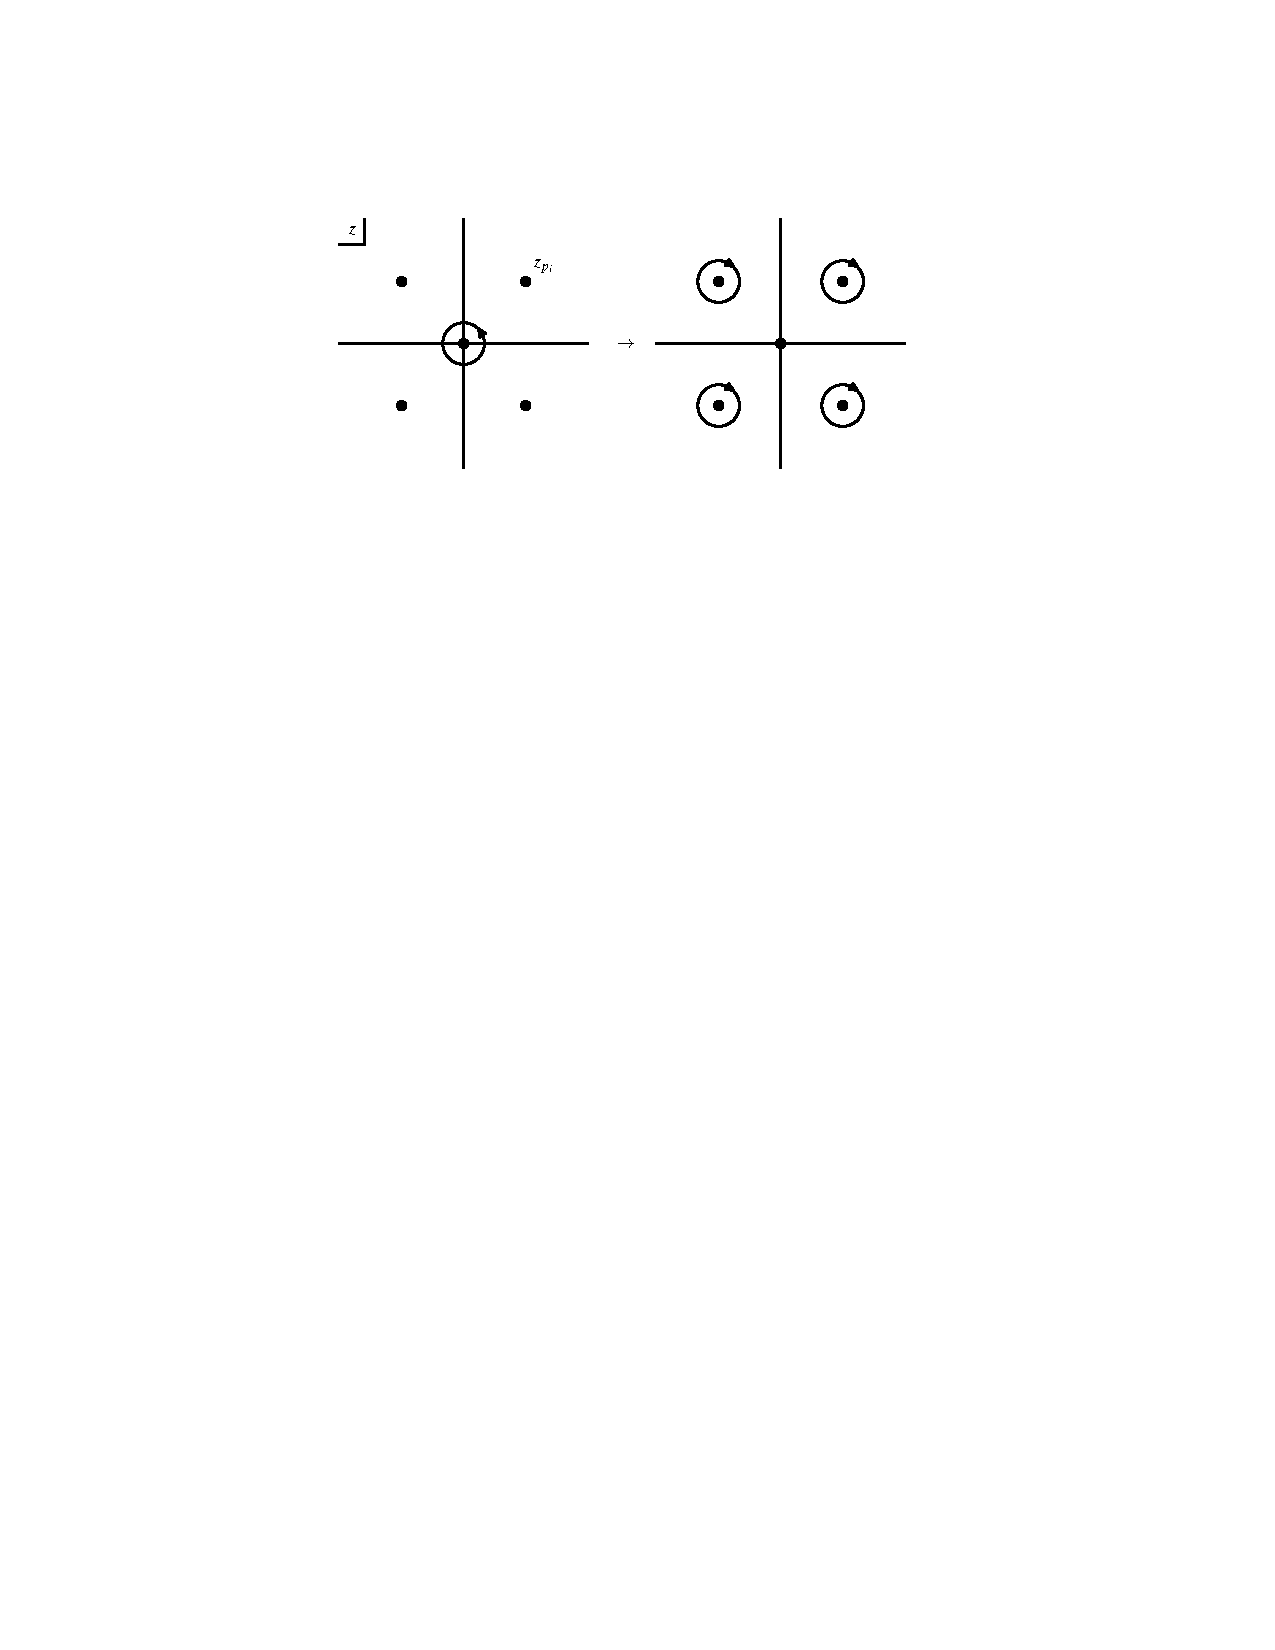
\includegraphics{ch2_trees/figures/chap2_bcfwpoles.pdf}
  \caption{
 Using Cauchy's theorem to obtain  
  eq.~(\ref{BCFWrec}) we may 
   pull the initial circle $C_{0}$ off to infinity thereby encircling the other poles
   clock-wise.} 
   \label{Fig:II.1}
\end{figure}
%
Here $C_{0}$ is a  small circle around  $z{=}0$ that only contains  the pole around the origin. To obtain \eqn{BCFWrec} we have deformed  this into a large circle at  infinity, 
now   encircling all the poles $z_{P_{i}}$ in the complex plane but  with  an opposite
orientation. See figure \ref{Fig:II.1}.
 If $A_{n}(z) \to 0$ as $z\to \infty$ we can drop the boundary term
${\rm Res}(z=\infty)$.
As we shall argue in a moment, this is the case for gauge theories under certain conditions.

\pagebreak
\begin{svgraybox}{\bf BCFW recursion relation for gluon amplitudes.}
With this assumption, we arrive at the BCFW recursion relation~\cite{ch2_Britto:2005fq}:
%
\begin{align}\begin{split}\label{eq-bcfw}
A_{n}(1,\ldots, n) =&
 \sum_{i=3}^{n-1} \sum_{h=\pm} A_{i}\Bigl(\hat{1}(z_{P_{i}}),2,\ldots, 
-\hat{P}_{i}^{-h}(z_{P_{i}})\Bigr) \\
& \quad \frac{\i}{P_{i}^2}\,  A_{n+2-i}\Bigl (\hat{P}^{h}_{i}(z_{P_{i}}),i,\ldots, n-1, \hat{n}(z_{P_{i}}) \Bigr ) \, , 
\end{split}
\end{align}
%
with $z_{P_{i}}$  defined in \eqref{zPidef}, and $P_{i}=p_{1}+p_{2}+\ldots + p_{i-1}$.
This relation is constructive: the amplitudes appearing on the right-hand side have lower 
multiplicity than the initial $A_n$. Hence, with the seed three-gluon amplitudes
\eqref{3pointmhv} and \eqref{3pointmhvbar}  we can bootstrap this relation to construct \emph{all} $n$-gluon
trees without using Feynman diagrams at all! 
Even more, our nuclei---the three-point amplitudes---were obtained from helicity
scaling arguments alone, as discussed in section~\ref{sec:helscale}. 
In this derivation we chose to shift two neighbouring legs
$\hat{1}$ and $\hat{n}$. In fact, one can also shift non-neighbouring legs or even more than two legs
to obtain alternative recursion relations, see e.g.~\cite{ch2_Risager:2005vk,ch2_Elvang:2008vz}.
\end{svgraybox}

An open issue is the vanishing of the boundary term in \eqref{BCFWrec}. For this we need to
have that 
\be
\frac{1}{2\pi \i}\oint_{\infty}\frac{dz}{z} \, {A_{n}(z)} =0\, , \ee
which in turns requires  a large-$z$ falloff of the amplitude as $A_{n}(z) {\sim} z^{-1}$.
In fact, the large-$z$ behaviour depends on the helicities of the shifted legs, and one can show that
\begin{align}
A\bigl(\hat{1}^{+},\hat{n}^{-}\bigr)\stackrel{z\to \infty }{\sim} \frac{1}{z} \, , \qquad
A\bigl(\hat{1}^{+},\hat{n}^{+}\bigr)\stackrel{z\to \infty }{\sim} \frac{1}{z} \, , \qquad
A\bigl(\hat{1}^{-},\hat{n}^{-}\bigr)\stackrel{z\to \infty }{\sim} \frac{1}{z} \, , \qquad
\end{align}
yet $A\bigl(\hat{1}^{-},\hat{n}^{+}\bigr)\!\stackrel{z\to \infty }{\sim}\!z^{3}$, which is then a forbidden $[n1\rangle$ shift.
In the following we show the first  relation; the other scalings are more technical to derive,
and may be found in~\cite{ch2_Arkani-Hamed:2008bsc}.

\subsection{Large $z$ falloff}

In order to estimate the large $z$ behaviour of generic tree-level amplitudes we
 perform an analysis based on Feynman graphs.
There are three sources for $z$ dependence in a generic colour-ordered amplitude: the propagators, the interaction vertices,
and the polarisation vectors. 
Consider a generic graph contributing to the tree-level $n$-gluon amplitude ($\hat{1}$ and $\hat{n}$ are assumed to be neighbours).
The $z$ dependence occurs only along the path from $\hat{1}$ to $\hat{n}$, see figure~\ref{fig:zscaling}.
Along this path, each three-gluon vertex, being linear in the momenta, maximally contributes a factor of $z$, while four-gluon vertices do not contribute, and all propagators along the path contribute a factor of $1/z$.
\begin{figure}[tt]
%%\fl
\begin{center}
$$
  \begin{tikzpicture}[baseline={(current bounding box.center)}]
  \begin{feynman}
    \coordinate (1) at (120:2);
    \coordinate (2) at (75:2);
    \coordinate (3) at (30:2);
    \coordinate (3b) at (5:1.8);
    \coordinate (4) at (-15:2);
    \coordinate (5) at (-60:2);
    \coordinate (6) at (-105:2);
    \coordinate (7) at (-150:2);
    \coordinate (8) at (-195:2);
    \coordinate (a) at (-1.0,0.75);
    \coordinate (b) at (-0.0,0.5);
    \coordinate (c) at (0.0,-0.5);
    \coordinate (d) at (1.0,-0.75);    
    \coordinate (e) at (0.75,1.15);    
    \coordinate (f) at (-0.75,-1.0);    
\diagram*{  (1) -- [gluon](a)};
\diagram*{  (8) -- [gluon](a)};
\diagram*{  (2) -- [gluon](e)};
\diagram*{  (3) -- [gluon](e)};
\diagram*{  (3b) -- [gluon](b)};
\diagram*{  (4) -- [gluon](d)};
\diagram*{  (5) -- [gluon](d)};
\diagram*{  (6) -- [gluon](f)};
\diagram*{  (7) -- [gluon](f)};
\draw [gluon]  (b) -- node [above] {$\frac{1}{z}$} (a);
\diagram*{  (b) -- [gluon](e)};
\draw [gluon] (b) -- node [left] {$\frac{1}{z}$}  (c);
\draw [gluon] (c) --  node [below] {$\frac{1}{z}$} (f);
\draw (f) node [above] {$z$};\draw (b) node [above] {$1$};
\draw (c) node [below] {$z$};
\draw (a) node [below] {$z$};
\diagram*{  (c) -- [gluon](d)};
  \draw (1) node [above] {$n-1$};
  \draw (2) node [above] {$n-2$};
%  \draw (3) node [right] {$4$};
%  \draw (4) node [right] {$6$};
  \draw (5) node [below] {$3$};
  \draw (6) node [below] {$2$};
  \draw (7) node [left] {$\hat{1}$};  
  \draw (8) node [left] {$\hat n$};
    \draw [loosely dotted, line width=1.5pt] (25:2.2) to[bend left=40] (-10:2.2); 
       \draw [fill] (a) circle (.08);
       \draw [fill] (b) circle (.08);
      \draw [fill] (c) circle (.08);
      \draw [fill] (d) circle (.08);
       \draw [fill] (e) circle (.08);
      \draw [fill] (f) circle (.08); 
      \end{feynman}      
              \end{tikzpicture}
$$
\end{center}
\caption{
The $z$ scaling of a generic graph: along the path from $\hat{1}$ to $\hat n$ the propagators
scale as $1/z$, the three-point vertices as $z$, while four-point vertices do not scale. 
This sample graph scales as $1$. However, if we
would replace the four-point vertex by a three-point one, it would scale as $z$.
On top of that we have to consider the $z$ scaling of the polarisation vectors.
}
\label{fig:zscaling}
\end{figure}
We may derive an upper bound for the $z$-scaling by considering the diagrams with maximal powers of $z$.
This happens when the path from $\hat{1}$ to $\hat{n}$ contains \emph{only} three-valent vertices. 
In that case it is easy to see that the graph scales as $z$:
\be
\begin{tikzpicture}[baseline={(current bounding box.center)}, scale = 0.9]
\begin{feynman}
\coordinate (1) at (-2,0);
\coordinate (2) at (-1,1);
\coordinate (a2) at (-1,0);
\coordinate (3) at (0,1);
\coordinate (a3) at (0,0);
\coordinate (4) at (1,1);
\coordinate (a4) at (1,0);
\coordinate (a5) at (2,0);
\coordinate (a6) at (3,0);
\coordinate (n-1) at (4,1);
\coordinate (an-1) at (4,0);
\coordinate (n) at (5,0);
\draw [gluon] (1) -- (a2);
\draw [gluon] (a2) to node[below]{$\frac{1}{z}$}  (a3);
\draw [gluon]  (a3) to node[below]{$\frac{1}{z}$} (a4);
\draw [gluon] (a6) to node[below]{$\frac{1}{z}$} (an-1);
\draw [gluon] (a4) to node[below]{$\frac{1}{z}$} (a5);
\draw [gluon] (2) -- (a2);
\draw [gluon] (3) -- (a3) ;
\draw [gluon] (4) -- (a4) ;
\draw [gluon] (n-1) -- (an-1) ;
\draw [gluon] (n) -- (an-1) ;
\draw (-1,0) node [below] {z};
\draw (0,0) node [below] {z};
\draw (1,0) node [below] {z};
\draw (2,0) node [below] {z};
  \draw (a5) node [right] {$\ldots\ldots$};
  \draw (1) node [left] {$\hat 1$};
            \draw (n) node [right] {$\hat{n}$};  
        \draw [fill] (an-1) circle (.08);
       \draw [fill] (a2) circle (.08);
         \draw [fill] (a3) circle (.08);
       \draw [fill] (a4) circle (.08);  
             \draw [fill] (an-1) circle (.08);  
             \end{feynman}
\end{tikzpicture}
\sim z \,.
\ee
Finally, there is an additional $z$ dependence arising from the polarisation vectors at legs $1$ and $n$:
\begin{eqnarray}
\epsilon_{1}^{+ \alpha \dot{\alpha}} &=& - \sqrt{2} \, \frac{ \tilde{\lambda}_{1}^{\dot\alpha} \mu_{1}^{\alpha}}{ \vev{ \hat{\lambda}_{1}(z) \mu_{1}}}  \sim \frac{1}{z} \,, \qquad 
\epsilon_{1}^{- \alpha \dot{\alpha}} = \sqrt{2} \, \frac{ {\hat{\lambda}_{1}}^{\alpha}(z) \tilde\mu_{1}^{\dot\alpha}}{ \lbrack \lambda_{1} \mu_{1} \rbrack } \sim z \,,  \\
%
%
\epsilon_{n}^{+ \alpha \dot{\alpha}} &=& - \sqrt{2} \, \frac{ 
\hat{\tilde{\lambda}}_{n}^{\dot\alpha}(z)
 \mu_{n}^{\alpha}}{ \vev{ \lambda_{n} \mu_{n}}}  \sim z \,, \qquad 
\epsilon_{n}^{- \alpha \dot{\alpha}} = \sqrt{2} \, \frac{ {\lambda}_{n}^{\alpha} \tilde\mu_{n}^{\dot\alpha}}{ \lbrack \hat{\lambda}_{n}(z) \mu_{n} \rbrack } \sim \frac{1}{z} \,.
\end{eqnarray}
Therefore, taking all sources of $z$ dependence into account, 
we conclude that individual graphs scale at worst as
\begin{align}
\label{zshiftscaling}
\begin{alignedat}{2}
& A\bigl( \hat{1}^{+}, \hat{n}^{-}\bigr) \stackrel{z\to \infty }{\sim} \frac{1}{z} \,, \qquad \qquad && A\bigl( \hat{1}^{+}, \hat{n}^{+} \bigr) \stackrel{z\to \infty }{\sim} z\,,\\
& A\bigl( \hat{1}^{-}, \hat{n}^{-}\bigr) \stackrel{z\to \infty }{\sim} z \,, \qquad \qquad  && A\bigl( \hat{1}^{-},\hat{n}^{+} \bigr) \stackrel{z\to \infty }{\sim} z^3\,. \\
\end{alignedat}
\end{align}
This shows that the $[-+\rangle$-shift has the desired falloff properties that allow us to drop the boundary term
at infinity in the BCFW formula~\eqref{eq-bcfw}. By cyclicity, it is always possible to find a $\{ \hat{1}^{+} , \hat{n}^{-} \}$ 
pair.
In fact, the above bound is too conservative. It was shown in~\cite{ch2_Arkani-Hamed:2008bsc}
that the $[++\rangle$ and $[--\rangle$-shifts also lead to an overall ${1}/{z}$ scaling once the sum over all Feynman graphs is performed, as the terms scaling as $z$ or $1$ cancel out.
Only the $[+-\rangle$-shift gives a non-vanishing $\text{Res}(z={\infty})$ in general, and may not be used as basis for a BCFW recursion.


\section{BCFW recursion for gravity and other theories}

Can we generalise the BCFW recursion to other \emph{massless} quantum field theories? If we 
analyse its
derivation in section \ref{sec:2.2}, we see that only two ingredients were  needed to establish it:
\begin{enumerate}
\item Tree-level amplitudes factorise on simple poles
whenever the square of the sum of a subset of external momenta vanishes. While for colour-ordered amplitudes we only need to consider adjacent channels, this is not essential for
the derivation of the BCFW recursion: factorisation is a completely general property, and that
is all that is needed.
\smallskip
\item The deformed amplitude $A_{n}(z)$ falls off as $1/z$ at infinity. This depends on the theory and is related to its ultraviolet  behaviour.
\end{enumerate}
Therefore, in order to construct 
tree-level amplitudes recursively without colour ordering from their factorisation properties, we need to
consider all multi-particle channels that may occur. We thus generalise the region momenta to include any subset $I$ of the momenta $\{p_1,\ldots,p_n\}$,
\be
P_{I}^{\mu}\coloneqq\sum_{i\in I}p_{i}^{\mu} \,.
\ee
Whenever  $P_{I}^{2}=0$ we have a pole, and, if a two-particle BCFW shift is used, the set $I$ must contain only one of the shifted momenta so that $P_{I}^{2}$ becomes $z$-dependent.
Concretely, the BCFW recursion
for a shift of legs $1$ and $n$ as in \eqn{bcfw-n1}
in gravity takes the form~\cite{ch2_Bedford:2005yy, ch2_Cachazo:2005ca}
%
\begin{align}\label{eq-bcfw-grav}
M_{n} =  
 \sum_Q \sum_{h=\pm\pm} %&
 M_L\Bigl(\hat{1}(z_{P_{Q}}),Q, 
-\hat{P}_{Q}^{-h}(z_{P_{Q}})\Bigr)
%\times %\\ &\times 
\frac{\i}{P_{Q}^2}\,  M_{R}\Bigl (\hat{P}^{h}_{Q}(z_{P_{Q}}),\bar{Q}, \hat{n}(z_{P_{Q}}) \Bigr ) \,,
%\nonumber
\end{align}
%
where the first sum runs over \emph{all} subsets $Q$ of momenta in  $\{p_{2},\ldots, p_{n-1}\}$, $\bar{Q}$ is the complement of $Q$, and
$P_{Q}=p_{1}+\sum_{i\in Q}P_{i}$.
Again, the recursion is only valid for the $[n1\rangle$ shifts
%
\be
\label{thisonep}
|\hat 1\rangle = |1\rangle - z |n\rangle\, , \qquad
|\hat n] = |n] + z |1]\, ,
\ee
%
of the types $[-+\rangle$, $[++\rangle$, and $[--\rangle$. For a derivation
see~\cite{ch2_Arkani-Hamed:2008bsc}.

Finally, we note that the BCFW recursion can be  generalised to massive theories~\cite{ch2_Badger:2005zh,ch2_Badger:2005jv} to be discussed in section~\ref{sec:2.6}, to 
the rational parts of one-loop amplitudes in QCD and gravity~\cite{ch2_Bern:2005hs,ch2_Bern:2005ji,ch2_Brandhuber:2007up,ch2_Dunbar:2010xk,ch2_Alston:2015gea} and form factors~\cite{ch2_Brandhuber:2010ad,ch2_Brandhuber:2011tv}. In supersymmetric Yang-Mills theory a
supersymmetric  version of the BCFW recursion may be formulated~\cite{ch2_Brandhuber:2008pf,ch2_Arkani-Hamed:2008owk}. In fact this recursion could be solved analytically~\cite{ch2_Drummond:2008cr}. 

\section{MHV amplitudes from the BCFW recursion relation}
\label{sect:MHVfrom BCFW}

\subsection{Proof of the Parke-Taylor formula}

As an application of the colour-ordered BCFW recursion~\eqref{eq-bcfw}, we  now derive  the   Parke-Taylor formula~\eqref{ParkeTaylor1} for MHV amplitudes.  
We already know from  section~\ref{sec:1.10} that it  is true for $n=3$ and $n=4$ through an explicit computation.
Therefore we shall prove by induction that the formula is correct. 
We focus here on the case where particles $n$ and $1$ have negative helicity, and 
perform  the $[n1\rangle$ shifts of \eqn{bcfw-n1}. The MHV amplitude has no multi-particle factorisation, as was discussed in section~\ref{sect:collinear}. Hence, only the two BCFW diagrams of
figure~\ref{Fig:MHVproof} contribute to the BCFW recursion of \eqn{eq-bcfw}.
%
\begin{figure}[t]
\begin{center}
\begin{equation*}
  \begin{tikzpicture}[baseline={(current bounding box.center)}, scale = 0.87]
  \begin{feynman}
  \coordinate (i) at (40:2.5);
\coordinate (n-1) at (-20:3.1);
\coordinate (n) at (-40:2.7);
\coordinate (1) at (-140:2.5);
\coordinate (2) at (150:2.9);
\coordinate (x) at (-1.5,0);
\coordinate (y) at (1.5,0);
\draw [gluon, momentum=$P$] ( 0.8,0) to  ( -0.8,0);
\draw [gluon] (x) -- ( 1);
\draw [gluon] (x) -- (2);
\draw [gluon] (y) -- (i); 
\draw [gluon] (y) -- (n); 
\draw [gluon] (y) -- (n-1); 
  \draw (1) node [below] {$\hat{1}^{-}$};
  \draw (2) node [left] {$2^{+}$};
  \draw (n) node [below] {$\hat{n}^{-}$};
    \draw (n-1) node [right] {$(n-1)^{+}$};
        \draw (i) node [above] {$3^{+}$};
         \draw ( -0.8,0.3) node [right] {$+$};            
   \draw ( 0.8,0.3) node [left] {$-$};
    \draw [loosely dotted, line width=1.5pt] (-10:2.5) to[bend right=50] (25:2.2);                        
 \draw [fill=lightgray,thick, draw=black] (x) circle (0.7);
 \draw (x) node {$\widebar{\text{MHV}}_{3}$};    
\draw [fill=lightgray,thick, draw=black] (y) circle (0.7);
 \draw (y) node {$\text{MHV}_{n-1}$};  
 \draw (0,-1.8) node {$(\text{I})$};  
\end{feynman}
\end{tikzpicture}
\, 
\begin{tikzpicture}[baseline={(current bounding box.center)}, scale = 0.87]
  \begin{feynman}
  \coordinate (i) at (140:2.5);
\coordinate (n-1) at (40:2.5);
\coordinate (n) at (-40:2.7);
\coordinate (1) at (-140:2.5);
\coordinate (2) at (-160:2.9);
\coordinate (x) at (-1.5,0);
\coordinate (y) at (1.5,0);
\draw [gluon, momentum=$P$] ( 0.8,0) to  ( -0.8,0);
\draw [gluon] (x) -- ( 1);
\draw [gluon] (x) -- (2);
\draw [gluon] (x) -- (i); 
\draw [gluon] (y) -- (n); 
\draw [gluon] (y) -- (n-1); 
  \draw (1) node [below] {$\hat{1}^{-}$};
  \draw (2) node [left] {$2^{+}$};
  \draw (n) node [below] {$\hat{n}^{-}$};
    \draw (n-1) node [right] {$(n-1)^{+}$};
        \draw (i) node [above] {$(n-2)^{+}$};
         \draw ( -0.8,0.3) node [right] {$-$};            
   \draw ( 0.8,0.3) node [left] {$+$};
    \draw [loosely dotted, line width=1.5pt] (-170:2.5) to[bend left=50] (150:2.2);                        
 \draw [fill=lightgray,thick, draw=black] (x) circle (0.7);
 \draw [fill=lightgray,thick, draw=black] (y) circle (0.7);
 \draw (y) node {$\widebar{\text{MHV}}_{3}$};    
 \draw (x) node {$\text{MHV}_{n-1}$};  
 \draw (0,-1.8) node {$(\text{II})$};  
\end{feynman}
\end{tikzpicture}
%
 \end{equation*}
\end{center}
\vspace*{-2mm}
\caption{
The two BCFW diagrams contributing to the $\text{MHV}_{n}$ amplitude. In fact, diagram $(\text{II})$ does
not contribute.
}
\label{Fig:MHVproof}
\end{figure}
%
%
We recall the $[n1\rangle$ shift,
\bal{
\label{n1shiftrecap}
|\hat 1 \rangle &= |1\rangle - z |n\rangle\, , \quad
|\hat n ] = |n] + z |1]\, , \quad \hat P = P -z \, |n\rangle [1|\, ,
}
%
whereas $|\hat 1] = |1]$ and $|\hat n \rangle = |n\rangle$ are left inert.

In fact, diagram $(\text{II})$ does not contribute. Here, the right diagram is of $\widebar{\text{MHV}}_{3}$ type.
Its numerator reads $[\hat P | n-1]^{3}$, cf.~\eqn{3pointmhvbar}, which vanishes:
%
\be
[n-1|\hat P ] = \frac{[n-1|\hat P |n\rangle}{\vev{\hat P \, n}} =
\frac{[n-1|(P - z \, |1]\, \langle n|)|n\rangle}{\vev{\hat P \, n}} =
\frac{[n-1|P|n\rangle}{\vev{\hat P \, n}} \stackrel{P=-p_{n-1}-p_{n}}{=}
0 \,.
\ee
%
In fact, this vanishing is consistent with the observation that the
$\widebar{\text{MHV}}_{3}$ kinematical assumption of collinear left-handed spinors, i.e.~$\vev{(n-1)|\hat n}=\vev{(n-1)|n}=0$, 
forces the two momenta $p_{n-1}$ and $p_{n}$ to be collinear, $p_{n-1}\parallel p_{n}$.
This is an inconsistent assumption on the $n$-particle kinematics. This is not a problem
for diagram $(\text{I})$, where the analogue condition reads $\vev{2|\hat 1}=0$, which does not
imply collinearity of $p_{1}$ and $p_{2}$ as $|\hat 1\rangle \neq |1\rangle$. 

Therefore only the BCFW diagram $(\text{I})$ contributes, where $A_L$ is a three-point $\overline{\rm MHV}$ amplitude, and $A_R$ is an $(n-1)$-point MHV amplitude. 
From \eqn{zPidef}, the position of the pole is 
\begin{align}
z_{P} = \frac{ (p_1 + p_2 )^2 }{ \langle n | P|1 \rbrack} = \frac{ \vev{12}\lbrack2 1 \rbrack}{\vev{n 2} \lbrack2 1\rbrack} = \frac{\vev{12}}{\vev{n 2}} \, .
\end{align}
The amplitudes $A_{L}$ and $A_{R}$ are then given by
\begin{align} \begin{aligned}
& A_{L} = A^{\overline{\text{MHV}}}_{3}\bigl( \hat{1}^{-},2^{+},-\hat{P}^{+} \bigr) =  \i g  
\frac{ \lbrack 2 (-
\hat{P}) \rbrack^3}{\lbrack \hat{1}2 \rbrack \lbrack (-\hat{P}) \hat{1} \rbrack} \,, \\
& A_{R} = A^{\text{MHV}}_{n-1}\bigl(\hat{P}^- , 3^+ , 4^+, \ldots (n-1)^{+} , \hat{n}^{-}\bigr) =   -\i g^{n-3}  \frac{ \vev{\hat{n} \hat{P}}^3 }{\vev{\hat{P} 3} \vev{34} \cdots \vev{(n-1) \hat{n}}}\,.
\end{aligned} \end{align}
Using \eqref{negpspin}, the fact that $\lambda_n$ and $\tilde{\lambda}_1$ are not shifted in  our $[n1\rangle$ shift of \eqn{thisonep}, as well~as 
%
\begin{align}
\vev{\hat{n} \hat{P}} \bev{\hat P 2} &= \vev{n\hat 1}\, \bev{12} = \vev{n1}\, \bev{12}\, , \qquad
\vev{3\hat P}  \,\bev{\hat P 1} 
%&
= \vev{32}\, \bev{2\hat 1} = \vev{32}\, \bev{21}\, , 
\end{align}
%
we find
\begin{align} \begin{aligned}
A_{L}  \frac{\i}{(p_1 + p_2)^2} A_{R} &=
\i g^{n-2}\frac{\vev{n1}^{3}
\, \bev{12}^{3}}{\bev{12}\bev{21}\vev{32}\bev{21}\, \vev{12}\vev{34}\cdots
\vev{(n-1)\, n}} \\
&
=- \i g^{n-2} \frac{ \vev{n 1}^4}{\vev{12} \cdots \vev{n1}} \ , 
\end{aligned} \end{align}
in agreement with the conjecture~\eqref{ParkeTaylor1} for the chosen helicities. This proves
the Parke-Taylor formula for adjacent negative-helicity states.


\subsection{The four-graviton MHV amplitude}

As a second example using the BCFW recursion for non-colour-ordered amplitudes~\eqref{eq-bcfw-grav} we compute the four-graviton amplitude $M_{4}(1^{--},2^{--},3^{++},4^{++})$. For
this we perform a
$[2^{--}1^{--}\rangle$ shift,
%
\bal{
\label{n1shiftrecap}
|\hat 1 \rangle &= |1\rangle - z |2\rangle\, , \quad
|\hat 2 ] = |2] + z |1]\, .
}
%
As $M_{n}(--,++,\ldots,++)=0$ for $n>3$, we again only find two channels in the BCFW
recursion, as shown in fig.~\ref{Fig:MHVproof} with the hatted leg $\hat n$ now replaced by $\hat 2$,
while the positive-helicity legs are summed over. Still, the same argument for the vanishing of the
type-$(\text{II})$ diagrams applies. For the special case of the four-point graviton amplitude we therefore
have
%
\be
M_{4}(1^{--},2^{--},3^{++},4^{++})=
\begin{tikzpicture}[baseline={(current bounding box.center)}, scale = 0.95]
  \begin{feynman}
\coordinate (3) at (-1,-.7);
\coordinate (4) at (1,-.7);
\coordinate (1) at (-1,.7);
\coordinate (2) at (1,.7);
\coordinate (x) at (-0.7,0);
\coordinate (y) at (0.7,0);
\draw [graviton] (x) to node [below] {$P$} (y);
\draw [graviton] (x) to (1);
\draw [graviton] (x) to (3);
\draw [graviton] (y) to (2);
\draw [graviton] (y) to (4);
\draw [ghost, momentum',white] (-0.5,-.1) to (0.5,-0.1);
\draw (1) node [left] {${\hat 1}^{--}$};
\draw (2) node [right] {${\hat 2}^{--}$};
\draw (3) node [left] {$3^{++}$};
\draw (4) node [right] {$4^{++}$};
 \draw [fill] (y) circle (.08);
 \draw [fill] (x) circle (.08);
  \draw ( -0.7,0.3) node [right] {$++$};            
   \draw (0.7,0.3) node [left] {$--$};
\end{feynman}
\end{tikzpicture} + (3\leftrightarrow 4) \,,
\ee
%
with $P=-p_{1}-p_{3}$. Inserting the three-graviton amplitudes~\eqref{generalsMHV} this becomes (setting $\kappa = 1$)
%
\bal{
M_{4}(1^{--},2^{--},3^{++},4^{++}) &= \left ( \frac{\bev{\hat P 3}^{3}}{\bev{31}\bev{1\hat P}}\right ) ^{2} \frac{\i}{(p_{1}+p_{3})^{2}}
\left ( \frac{\vev{\hat P 2}^{3}}{\vev{24}\vev{4\hat P}}\right ) ^{2} + (3\leftrightarrow 4) \nn \\
&= \frac{\i}{s_{13}} \frac{\langle 2 | \hat P | 3]^{6}}{\vev{24}^{2}\bev{31}^{2}\langle 4| \hat P|1]^{2}}
+ (3\leftrightarrow 4) \,.
}
%
We now use $\hat P=p_{2}+p_{4} + z |2\rangle [1|$ to find $\langle 2 | \hat P | 3]=\vev{24}\bev{43}$ and
$\langle 4| \hat P|1]=\vev{42}\bev{21}$. Hence, the $z$ dependance drops out! Inserting these two relations
one finds
%
\be
M_{4}(1^{--},2^{--},3^{++},4^{++}) = \i \frac{\bev{34}^{6}}{\bev{12}^{2}}
\left( \frac{\vev{24}^{2}}{\vev{13}\bev{31}^{3}} + \frac{\vev{23}^{2}}{\vev{14}\bev{41}^{3}} \right ) \, ,
\ee
where $s_{ij} = (p_i+p_j)^2$.
While this is the final result, one may write it using the Mandelstam variables
%
\be
s=(p_{1}+p_{2})^{2}\, , \quad  t=(p_{2}+p_{3})^{2}\, ,  \quad u=(p_{1}+p_{3})^{2}\, .
\ee
Doing this one
finally arrives at the compact result (reinstating the coupling)
%
\be
\label{M4MHVfinal}
M_{4}(1^{--},2^{--},3^{++},4^{++})=\i \kappa^{2} \, \frac{\vev{12}^{4}\bev{34}^{4}}{stu} \,,
\ee
%
with a peculiar pole structure. The correct helicity scaling is easily checked.
Similarly to the gluon case, a closed expression for the MHV $n$-graviton tree-level amplitude may also be 
conjectured and proven via BCFW recursion. Yet, it is more involved and may be found in~\cite{ch2_Berends:1988zp}.


\begin{exer}{The six-gluon split-helicity NMHV amplitude}
\label{Ex:6gNMHV}
Determine the first non-trivial next-to-maximally-helicity-violating (NMHV) amplitude 
$$A_{6}^{\rm tree}(1^{+}, 2^{+}, 3^{+}, 4^{-}, 5^{-}, 6^{-} )$$
from a BCFW recursion relation and our knowledge of the
MHV amplitudes. Consider a shift of the two helicity states $1^{+}$ and $6^{-}$, and show that
\begin{align} \label{eq:A6NMHV}
\begin{aligned}
A_{6}^{\text{tree}}(1^{+},2^{+},3^{+}, 4^{-},& 5^{-},6^{-}) = 
\i g^4 \biggl( \frac{\langle6|P_{12}|3]^{3}}{\vev{61}\vev{12}\bev{34}\bev{45}[5|P_{16}|2\rangle }
 \frac{1}{ (p_{6}+p_{1}+p_{2})^{2}} \\
& \phantom{=} + \frac{\langle 4 | P_{56}|1]^{3}}{ \vev{23}\vev{34}\bev{16}\bev{65}[5|P_{16}|2\rangle} 
\frac{1}{ (p_{5}+p_{6}+p_{1})^{2}} \biggl) \, , 
\end{aligned}
\end{align}
%
where $P_{ij}=p_{i}+p_{j}$. 
For the solution see \hyperref[Sol:6gNMHV]{chapter~5}.
\end{exer}


\begin{exer}{Soft limit of the six-gluon split-helicity amplitude}
\label{Ex:6gSoft}
Check the consistency of the six-gluon split-helicity amplitude of \eqn{eq:A6NMHV} with the soft limit of leg $5$.
For the solution see \hyperref[Sol:6gSoft]{chapter~5}.
\end{exer}



\section{BCFW recursion with massive particles}
\label{sec:2.6}

So far we restricted our attention to amplitudes involving massless particles,
i.e.~gluons, gravitons, and massless fermions and scalars. 
Yet, scattering amplitudes involving massive particles are of great relevance
in physics, and consequently on-shell recursions have been devised for this case as well.
Let us focus here on colour-ordered gauge-theory amplitudes involving also massive
coloured matter fields (for the colour-ordered amplitudes the representation of the matter
field is irrelevant). Concretely, we consider amplitudes involving at least two massless gluons,
which we take to be neighbours for simplicity of the discussion, say at positions $1$ and $n$,
together with $n-2$ massive states:
%
\be
A_{n}(p_{1},p_{2},\ldots, p_{n})\, , \qquad  p_{1}^{2}=0=p_{n}^{2}\, ,
\qquad p_{i}^{2}=m_{i}^{2} \, .
\ee
%
Let us now see how the BCFW on-shell recursion
derived in section \ref{sec:2.2} may be generalised to gauge theory
amplitudes with massive particles. We closely follow reference~\cite{ch2_Badger:2005zh}
in our exposition.

As before in \eqn{bcfw-n1}, we consider a complex shift  of the null gluon  momenta 
at positions $1$ and $n$  by a parameter $z\in \mathbb{C}$,
%
\be
{\hat p}_{1}(z)   = p_{1} - z |n\rangle [1| \, , \qquad
{\hat p}_{n}(z)   = p_{n} + z |n\rangle [1| \, .
\ee
%
This entails a $z$-shift of the region momentum $P_{i} \coloneqq p_{1}+\ldots p_{i-1}$,
\be
{\hat P}_{i}(z)  = P_{i} - z |n\rangle [1| \, ,  \qquad i\in \{3,\ldots , n-1\}\, ,
\ee
which also featured in the BCFW recursion
relation of \eqn{poleargumentbcfw}. 
Importantly, the on-shellness of the deformed legs $\hat 1$ and $\hat n$ as well as total momentum conservation is preserved under the shift.
As the arguments leading to the BCFW recursion 
relation are purely based on factorisation, they are applicable to a generic quantum field theory involving massive particles as well.
The BCFW recursion was obtained by thinking about the deformed amplitude 
$A_{n}(z)$ as an analytic function in $z$. Its poles arise whenever an internal propagator
associated to the $z$-shifted region momentum ${\hat P}_{i}(z)$ goes on-shell. 
This reasoning does not change in the massive case, i.e.~we will have a pole whenever 
a $z$-shifted region momentum goes on-shell, i.e.~$\hat P^{2}_{i}(z)=m^{2}$ with $i\in\{3,\ldots , n-1\}$ . 
The pole then reads in generalisation of \eqn{poleargumentbcfw} as
%
\begin{align}
\label{massivepoleargumentbcfw}
\frac{1}{\hat{P}_{i}(z)^{2}-m_{P_{i}}^{2}} & = \frac{1}{(\hat{p}_{1}(z) + p_{2} + \ldots p_{i-1})^2
-m_{P_{i}}^{2}} \nn \\ 
%
& = \frac{1}{P_{i}^2 -m_{P_{i}}^{2} - z \langle n | P_{i} | 1 \rbrack}\,, 
\end{align}
%
where $m_{P_{i}}$ is the mass of the associated intermediate particle going on-shell. 
Generalising \eqn{zPidef}, the location of the pole is shifted to
%
\be
\label{mzpole}
z_{P_{i}} =\frac{P_{i}^2-m_{P_{i}}^{2}}{\langle n | P_{i} | 1 \rbrack}\, , \qquad
\forall i \in \{3,\ldots , n-1\}\, . 
\ee
%
\begin{svgraybox}{\bf BCFW recursion relation with massive particles.}
Using again the complex analysis arguments of figure \ref{Fig:II.1}, one immediately arrives
at the on-shell recursion relation for amplitudes including massive particles:
%
\begin{align}
%
\begin{split}\label{massiveBCFWrec}
A_{n}(1,\ldots, n)  
= \sum_{i=3}^{n-1} \sum_{s \in s_{\rm P}}  &\, 
%
A_{L}\bigl(\hat 1(z_{P_{i}}),2,\ldots,i-1,-{\hat P}^{\bar{s}}(z_{P_{i}}) \bigr) 
\frac{\i \, n_{\rm P}}{P_{i}^2-m_{P_{i}}^{2}} \\ 
& \times A_{R}\bigl({\hat P}^{s}(z_{P_{i}}),i,\ldots, n-1, \hat n(z_{P_{i}})\bigr)
+ {\rm Res}(z=\infty)\,,
\end{split}
\end{align}
%
where the sum now is over the spins $s_{\rm P}$ of the intermediate particle $\rm P$ and $n_{\rm P}$ is the particle-dependent constant appearing in the factorisation as described below \eqn{eq:multiparticlepole}. We recall
that the legs $1$ and $n$ are assumed to be massless. 
\end{svgraybox}

Again, this formula is only of use if 
the residue at infinity, ${\rm Res}(z=\infty)$, vanishes. This turns out to be the case if the
gluon helicities of the shifted legs are not of the $[n^{+}1^{-}\rangle$ type, just as in 
\eqn{zshiftscaling}. Hence, the
statement is
%
\be
{\rm Res}(z=\infty)=0 \quad \text{iff}\quad 
(h_{1},h_{n})= (+,-)\, , \, (+,+)\, , \, (-,-)\, .
\ee
%
See~\cite{ch2_Badger:2005zh} for a derivation. This renders the massive BCFW
recursion relation~\eqref{massiveBCFWrec} very useful.



\subsection{Four-point amplitudes with gluons and massive scalars}

Let us construct an explicit example. We consider a theory of a massive complex 
scalar field coupled to gauge theory.
Concretely, we want to evaluate the four-point amplitude involving two neighbouring
gluons of positive helicity and two scalars, 
%
\be
\label{ggpp}
A_{4}(1^{+},2_{\phi},3_{\bar\phi},4^{+})\, .
\ee
%
The scalars have mass $m^{2}$. This amplitude vanishes
in the massless limit $m=0$, similarly to the vanishing of
the above amplitude when the scalars are replaced by massless fermions, as was
shown in \eqn{I.32}.  In fact, amplitudes of the above type are of interest even
in massless theories at the one-loop level. There, the need to 
regulate divergences leads one to consider internal particles propagating
in $D=4-2\epsilon$ dimensions which may be modelled using masses, as we shall discuss in detail in the next chapter.

Returning to our concrete example we employ the massive on-shell recursion 
of \eqn{massiveBCFWrec}. Only the scalar
channel contributes, 
%
\be
\label{massive4rec}
A_{4}(1^{+},2_{\phi},3_{\bar\phi},4^{+})=
A_{3}\bigl(\hat 1^{+}, 2_{\phi}, -{\hat P}_{\bar\phi}\bigr)\, \frac{\i}{P^{2}-m^{2}}\,
A_{3}\bigl({\hat P}_{\phi},3_{\bar\phi},\hat{4}^{+}\bigr) \,,
\ee
%
as an amplitude with a single scalar vanishes, $A_{3}(\hat 1^{+}, 2_{\phi},3^{\pm})=0$.
All that is needed are the $(\phi g \bar\phi)$-amplitudes.
These follow from the colour-ordered Feynman
vertices of two charged scalars and a gluon of \eqn{cOsQCD},
%
\be
V_{3}(l_{1},p^{\mu},l_{2})=
\raisebox{-0.6cm}{\begin{tikzpicture}
\begin{feynman}
	\coordinate (x) at (-0.7,0);
	\coordinate (o) at (0,0);
	\coordinate (y) at (0.75,0);
		\coordinate (z) at (0,-0.7);
		\diagram*{(x) -- [charged scalar] (o) -- [charged scalar] (y), (o) -- [gluon] (z)};
		\draw [fill] (x) circle (.0) node [left] {$l_{1}$} ;
	\draw [fill] (y) circle (.0) node [right] {$l_{2}$} ;
	\draw [fill] (o) circle (.06);
		\draw [fill] (z) circle (.0) node [right] {$\mu$} node [left] {$p$};
    \end{feynman}
	\end{tikzpicture}}
= \i \frac{g}{\sqrt{2}}\, (l_{2}^{\mu}-l_{1}^{\mu})\, ,
\ee
%
where $1$ ($2$) denotes a $\bar\phi$ ($\phi$) leg, respectively.
Contracting this with the positive-helicity gluon polarisation of \eqn{s1polarrel} one
obtains the on-shell three-point amplitudes (setting $g=1$)
%
\be
\label{ssp}
A_{3}(l_{1\, \bar{\phi}},p^+,l_{2 \, \phi})= -\i\frac{\langle r|l_{1}|p]}{\vev{rp}} =
A_{3}(l_{1\, {\phi}},p^+,l_{2 \, \bar\phi})\, ,
\ee
%
where the last relation follows by reflection.
Note that here $r$ is the arbitrary null reference 
momentum of the gluon leg related to the local gauge invariance of the theory.
By similar arguments one establishes the three-point amplitudes involving a negative
helicity gluon:
%
\be
\label{ssm}
A_{3}(l_{1\, \bar{\phi}},p^-,l_{2 \, \phi})=-\i \frac{\langle p|l_{1}|r]}{[pr]} =
A_{3}(l_{1\, {\phi}},p^-,l_{2 \, \bar\phi})\, .
\ee
%
Before moving on with the recursion, let us address a seemingly dramatic problem: 
the amplitudes of \eqn{ssp} and \eqn{ssm} apparently depend on the
reference momentum $r$---how can that be?
It turns out that, despite their representation, the amplitudes in \eqn{ssp} and \eqn{ssm}
are actually \emph{independent} of the choice of $r$. Taking the initial reference spinor
$|r\rangle$ and $|p\rangle$ as a basis in Weyl spinor space, we may parametrise 
an arbitrary reference spinor different from $|r\rangle$ as $|r'\rangle = \alpha |r\rangle + \beta |p\rangle$. Clearly, \eqn{ssp} is invariant under rescaling of the reference spinor $|r\rangle \to 
\Lambda\, |r\rangle$, thus without loss of generality
we may parameterise $|r'\rangle = |r\rangle + \gamma |p\rangle$, or  infinitesimally write
$\delta_{r}|r\rangle \propto |p\rangle$. This entails that the amplitude \eqn{ssp}  changes under
a variation of the reference spinor $|r\rangle$  as
%
\be
\delta_{r}A_{3}(l_{1}^{+},p^+,l_{2}^{-}) \propto \frac{\langle p|l_{1}|p]}{\vev{rp}}
=0 \, ,
\ee
%
where the vanishing follows from $\langle p|l_{1}|p]=2p\cdot l_{1}=0$, which is a consequence of 
the three-point kinematics:
%
\be
(l_{1}+p)^{2} = l_{2}^{2} \quad \rightarrow\quad  l_{1}\cdot p =0 \quad \text{as}
\quad l_{1}^{2}=l_{2}^{2}=m^{2}\, ,\,  p^{2}=0\, .
\ee
%
A similar argument applies to \eqn{ssm}. Again we see the subtleties in three-point amplitudes: the expressions in eqs.~\eqref{ssp} and~\eqref{ssm} are actually independent 
of $r$.
%
\begin{figure}[t]
   \centering
    \begin{tikzpicture}[baseline={(current bounding box.center)}]
  \begin{feynman}
  \coordinate (i) at (30:2.5);
\coordinate (n) at (-30:2.5);
\coordinate (1) at (-150:2.5);
\coordinate (2) at (150:2.5);
\coordinate (x) at (-1.2,0);
\coordinate (y) at (1.2,0);
\draw [charged scalar, momentum=$P$] ( 0.8,0) to  ( -0.8,0);
\draw [gluon] (x) -- ( 1);
\draw [charged scalar] (x) -- (2);
\draw [charged scalar] (i) -- (y); 
\draw [gluon] (y) -- (n); 
  \draw (1) node [below] {$\hat{1}^{+}$};
  \draw (2) node [above] {$2_{\phi}$};
  \draw (n) node [below] {$\hat{4}^{+}$};
           \draw (i) node [above] {$3_{\bar\phi}$};
 \draw [fill=lightgray,thick, draw=black] (x) circle (0.4);
 \draw (x) node {$A_{3}$};    
\draw [fill=lightgray,thick, draw=black] (y) circle (0.4);
 \draw (y) node {$A_{3}$};  
\end{feynman}
\end{tikzpicture}
   \caption{On-shell recursion for the massive 
   $A_{4}(1^{+},2_{\phi},3_{\bar\phi},4^{+})$ amplitude. All external momenta are
   outgoing, $P$ runs from right to left.}
   \label{fig:mss2}
\end{figure}
%

Coming back to the recursive construction of the amplitude $A_{4}(1^{+},2_{\phi},3_{\bar\phi},4^{+})$, we have
(cf.\ figure~\ref{fig:mss2})
%
\begin{align} \begin{aligned}
A_{4}(1^{+},2_{\phi},3_{\bar\phi},4^{+})&= A_{3}\bigl(-{\hat P}_{\bar\phi},\hat 1^{+},2_{\phi}\bigr)\, \frac{\i}{P^{2}-m^{2}}
\, A_{3}\bigl(3_{\bar\phi},\hat 4^{+},{\hat P}_{\phi} \bigr)\, \\
&= \left( \i \, \frac{\langle r_{1}|\hat P |\hat 1]}{\vev{r_{1}\hat 1}} \right) \frac{\i}{P^{2}-m^{2}} \left( - \i \,
 \frac{\langle r_{4}|p_{3}|\hat 4]}{\vev{r_{4}\hat 4}} \right) \,,
\end{aligned} \end{align}
%
with $P=p_{1}+p_{2}$.
Here $r_{1/4}$ denote the reference momenta of the gluon legs 1 and 4. Things are simplified
considerably with the gauge choice
%
\be
r_{1}=\hat p_{4}\, , \qquad r_{4}=\hat p_{1}\, .
\ee
%
Noting that $|\hat 1]=|1]$ and $|\hat 4 \rangle = |4\rangle$, we then have
%
\begin{align}
\begin{alignedat}{2}
& \langle r_{1}|\hat P|\hat 1] =  \langle 4|\hat P |1] = \langle 4|P|1] = - \langle 4|p_{3}|1] \, , \quad \quad
  && \vev{r_{1}\hat 1}=\vev{4\hat 1}=\vev{41}\, ,  \\
& \langle r_{4}|p_{3}|\hat 4] =  \langle \hat 1|p_{3} |\hat 4]\, , 
  && \vev{r_{4}\hat 4}=\vev{\hat 1 4 }=\vev{14}\, . \\
\end{alignedat} \end{align}
%
Plugging these into the above we find
%
\be
A_{4}= \i\frac{\langle 4 |p_{3}|1]\, \langle \hat 1 | p_{3}|\hat 4]}{\vev{14}^{2}\, 
[(p_{1}+p_{2})^{2} -m^{2}]}\, .
\ee
%
The numerator may be simplified with a trace identity (see \eqn{eq:trSigma2gamma}) to
%
\be
\langle 4 |p_{3}|1]\, \langle \hat 1 | p_{3}|\hat 4] = \frac{1}{2} \, \Tr \bigl(
\hat{\slashed{p}}_{4}\, \slashed{p}_{3} \,
\hat{\slashed{p}}_{1}\, \slashed{p}_{3} \,
 \bigr) = 2 \, \bigl ( \, 2 (p_{3}\cdot \hat p_{4})\, (p_{3}\cdot \hat p_{1})
 - p_{3}^{2}\, (\hat p_{1}\cdot \hat p_{4})\, \bigr )\, .
\ee
%
In fact $p_{3}\cdot \hat p_{4}=0$, which follows from momentum conservation:
%
\be
\hat P^{2} = (p_{3}+\hat p_{4})^{2}\quad \Rightarrow \quad
m^{2}= 2p_{3}\cdot \hat p_{4} + p_{3}^{2}\quad \Rightarrow \quad
p_{3}\cdot \hat p_{4}=0\, .
\ee
%
Moreover, we find $2\hat p_{1}\cdot \hat p_{4}=\vev{\hat 14}\bev{\hat 41}= \vev{14}\bev{41}$.
Putting everything together we arrive at the compact expression for the 
four-point amplitude
%
\be
\label{gpgpss}
A_{4}(1^{+},2_{\phi},3_{\bar\phi},4^{+})= \i \, \frac{\bev{14} \, m^{2}}{\vev{14}\,
[(p_{1}+p_{2})^{2} -m^{2}]}\, ,
\ee
%
which indeed vanishes in the massless limit, as claimed. 

\vspace{-0.1cm}

\begin{exer}{Mixed-helicity four-point scalar-gluon amplitude}
\label{Ex:2.helicity}
Compute the four-point massive-scalar-gluon amplitude with one positive and one negative gluon,
\begin{align}
A_{4}(1^{+},2_{\phi},3_{\bar\phi},4^{-}) =  \i \,
\frac{\langle 4| p_{3}| 1]^{2}}{ (p_1+p_4)^2 \, [(p_1+p_2)^2-m^2] } \,,
\end{align}
using the above recursive techniques. 
For the solution see \hyperref[Sol:2.helicity]{chapter~5}.
\end{exer}

\section{Symmetries of scattering amplitudes}
\label{sec:2.4}

We now turn to a more conceptual yet very  important subject: the question of how the
space-time symmetries of the Poincar\'e group (and beyond) that we discussed in section~\ref{sec:1.1} manifest themselves at the level of
scattering amplitudes. This has proven to be a very rich subject
in particular at tree level. The space-time symmetries of scattering amplitudes may be
grouped into obvious and less obvious symmetries.

The obvious symmetries are the Poincar\'e 
transformations of section~\ref{sec:1.1}, under which scattering amplitudes should be invariant. 
Sticking to massless amplitudes,  working in the spinor-helicity formulation of momentum space 
is highly advantageous. Here
the momentum generator $p^{\a\da}$ is represented by a multiplicative operator,
%
\begin{align}
p^{\a\da} & = \sum_{i=1}^n \la_i^\a \, \tla_i^\da\, , \quad
\end{align}
%
and any amplitude $\cA_n$ must obey
%
\be
p^{\a\da}\, \cA_n(\{\la_i,\tla_i\}) = 0\, .
\ee
%
This is in fact true in the distributional sense of the relation
$
p\, \delta(p)=0\,,
$
thanks to the total momentum conserving
delta-function present in each amplitude (that we often drop):
\be
 \cA_n(\la_i,\tla_i)=\delta^{(4)}\biggl(\sum_i p_i\biggr) \, A_n \left(\la_i,\tla_i \right) \,.
\ee
In our notation we distinguish the full amplitude $\cA_{n}$ and the delta-function ``stripped'' amplitude~$A_{n}$.

The Lorentz generators in the helicity spinor basis
come in two pairs of symmetric rank-two tensors
$m_{\a\b}$ and ${\overline m}_{\da\db}$, originating from the projections
$M^{\mu\nu}\, (\sigma_{\mu\nu})_{\a\b} = m_{\a\b}$ and 
$M^{\mu\nu}\, (\bar\sigma_{\mu\nu})_{\da\db} ={{\overline m}}_{\da\db}$.
They are first-order differential operators
in helicity spinor space,
%
\be
m_{\a\b} = \sum_{i=1}^n \la_{i\, (\a}\, \partial_{i\,\b)}\, , \quad
{{\overline m}}_{\da\db} = \sum_{i=1}^n \tla_{i\, (\da}\, \partial_{i\, \db)}\, ,
\ee
%
where $\partial_{i\a} \coloneqq \frac{\partial}{\partial \la_i^\a}$, 
$\partial_{i\da} \coloneqq \frac{\partial}{\partial \tla_i^\da}$ and
$r_{(\a\b)} \coloneqq (r_{\a\b} + r_{\b\a})/2$ denotes symmetrisation
with unit weight, cf.~exercise \ref{Ex:1.5}.
The invariance of $A_n(\la_i,\tla_i)$ under Lorentz-transformations,
%
\be
m_{\a\b}\, A_n(\la_i,\tla_i) = 0 = {{\overline m}}_{\da\db}\, A_n(\la_i,\tla_i)\,,
\ee
%
is manifest, as it is an immediate consequence of the proper 
contraction of all Weyl indices within $A_n$, i.e.~the fact
that the spinor brackets $\vev{ij}$ and $\bev{ij}$ are invariant under $m_{\a\b}$
and ${{\overline m}}_{\da\db}$. See the solution of exercise~\ref{Ex:1.5} for an explicit
calculation.

Let us now discuss a set of less obvious symmetries of $\cA_n(\la_i,\tla_i)$ in the
case of pure colour-ordered gluon amplitudes. Classical
Yang-Mills theory is in fact invariant under a larger symmetry group than Poincar\'e: 
due to the absence of dimensionful parameters in the theory (the coupling
$g$ is dimensionless) pure
Yang-Mills theory (as well as massless QCD or scalar QCD) is invariant under a scale transformation,
%
\be
x^\mu \to \Lambda^{-1}\, x^\mu\, , \quad \text{respectively} \quad
p^\mu \to \Lambda\, p^\mu\, .
\ee
%
The scale transformations of the momenta are generated by the dilatation operator $d$,
whose representation in spinor-helicity variables acting on amplitudes is
%
\be
d= \sum_{i=1}^n\, \left( \frac{1}{2} \la^\a_i\, \partial_{i\,\a} + 
 \frac{1}{2} \tla^\da_i\, \partial_{i\,\da} + d_0 \right) \,, \qquad d_0 \in \R \,,
\label{d_def}
\ee
%
reflecting the mass dimension $\nicehalf$ of the $\la_i$ and $\tla_i$ helicity spinors, 
i.e.~$[d,\lambda_i]=\lambda_i/2$ and $[d,\tla_i]= \tla_i/2$.
The constant $d_0$ is undetermined at this point. It may be fixed by requiring invariance
of the MHV gluon amplitudes,
%
\be
\cA_n^\text{MHV} =  \delta^{(4)}(p)\, \frac{\vev{st}^4}
{\vev{12}\ldots\vev{n1}}\, ,
\ee
%
where $p = \sum_{i=1}^n p_i$.
The dilatation operator $d$ of \eqn{d_def} simply measures the weight in units of mass
of the amplitude it acts on adding a factor of $n\, d_0$, namely
%
\be
d\, \cA_n = \bigl([\cA_n] + n\, d_0 \bigr)\, \cA_n \, ,
\ee
%
where $[\mathcal{O}]$ indicates the weight of $\mathcal{O}$ in dimensions of mass.
We note the weights $[\delta^{(4)}(p)]=-4$, $[\vev{st}^4]=4$ and
$[\vev{12}\ldots\vev{n1}]=n$, hence
%
\be
d\, \cA_n^\text{MHV} = (-4 + 4-n +n\, d_0) \, \cA_n^\text{MHV} \, ,
\ee
%
which vanishes for the choice $d_0=1$. 
One easily checks the invariance under dilatations of the $q\bar q gg$-amplitude of 
\eqn{qqgg-amp} and of the $\widebar{\text{MHV}}{}_n$ amplitudes as~well.

The scaling symmetry comes with a further less obvious symmetry of vectorial nature
known as special conformal transformations. Their generators, denoted by $k_{\a\da}$, are
realised in terms of a second-order differential operator in the spinor variables,
%
\be
k_{\a\da}= \sum_{i=1}^n \partial_{i\, \a}\, \partial_{i\, \da} \, .
\ee
%
Together with the Poincar\'e and dilatation
generators, the set $\{p_{\a\da}, k_{\a\da}, m_{\a\b}, {{\overline m}}_{\da\db}, d\}$ generates
the \emph{conformal group} in four dimensions, $\text{SO}(2,4)$.

Let us now prove the invariance of the MHV gluon amplitudes under special conformal
transformations. As the only dependence of $\cA^\text{MHV}_n$ on the conjugate
spinors $\tla_i$ resides in the momentum conserving delta-function, we have
%
\begin{align}
k_{\a\da} \, \cA^\text{MHV}_n &= 
\sum_{i=1}^n \frac{\partial}{\partial \la^\a_i}\,\frac{\partial}{\partial \tla^\da_i}\,
\left (\delta^{(4)}(p)\, A^\text{MHV}_n \right) \nn \\ &= 
\sum_{i=1}^n \frac{\partial}{\partial \la^\a_i}\,
\left[
\frac{\partial p^{\b\db}}{\partial\tla_i^\da}\, \left( \frac{\partial}{\partial p^{\b\db}}
\,\delta^{(4)}(p)\, \right) \, A_n^\text{MHV}\right]  \nn\\
&= \biggl [ \biggl( n\, \frac{\partial}{\partial p^{\a\da}} + p^{\b\db}\, 
\frac{\partial}{\partial p^{\b\da}} \, \frac{\partial}{\partial p^{\a\db}} \biggr)\, \delta^{(4)}(p)
\,   \biggr ] \, A^\text{MHV}_n \nn\\ &\qquad  + \biggl(\frac{\partial \,\delta^{(4)}(p)}{\partial p^{\b\da}}\biggr)\,
\sum_{i=1}^n\, \la_i^\b\, \frac{\partial}{\partial\la^\a_i}\, A_n^\text{MHV} \, .
\label{kAMHV}
\end{align}
%
The last term may be rewritten as follows. First, we note the relation
%
\be
\label{symlapa}
\sum_{i=1}^n\la_{i\, \a}\, \partial_{i\, \b} = \sum_{i=1}^n
\la_{i\, (\a}\, \partial_{i\, \beta)} + \frac{1}{2} \, \epsilon_{\a\b}\, \sum_i\la^\gamma_i\, 
\partial_{i\, \gamma} \, ,
\ee
%
which follows from decomposing the left-hand side in a symmetric and anti-symmetric piece.
The first term on the right-hand side is the Lorentz generator $m_{\a\b}$, which we already know annihilates
$A_n^\text{MHV}$. The remaining term yields
%
\be
\sum_{i=1}^n \la^\b_i\, \frac{\partial}{\partial\la^\a_i}\, A_n^\text{MHV}=
\frac{1}{2} \, \delta_\a^\b\, \sum_i \la^\delta_i\, \partial_{i\, \delta}\,  A_n^\text{MHV}=
(4-n)\, A_n^\text{MHV}\, .
\ee
%
Hence \eqn{kAMHV} turns into
%
\be
k_{\a\da} \, \cA^\text{MHV}_n =
\biggl [ \biggl( 4\, \frac{\partial}{\partial p^{\a\da}} + p^{\b\db}\, 
\frac{\partial}{\partial p^{\b\da}} \, \frac{\partial}{\partial p^{\a\db}} \biggr)\, \delta^{(4)}(p)
\,   \biggr] \, A^\text{MHV}_n \, .
\ee
%
Indeed in a distributional sense we have
%
\be
p^{\b\db}\, 
\frac{\partial}{\partial p^{\b\da}} \, \frac{\partial}{\partial p^{\a\db}}\, \delta^{(4)}(p)
=-4 \, \frac{\partial}{\partial p^{\a\da}}\, \delta^{(4)}(p)\, ,
\ee
%
which one may see by integrating the second derivative expression against a test function $F(p)$:
\begin{align} \begin{aligned}
\int \d^4 p &\, F(p)\, p^{\b\db}\, 
\frac{\partial}{\partial p^{\b\da}} \, \frac{\partial}{\partial p^{\a\db}}\, \delta^{(4)}(p)
= \\
&
= \int \d^4 p \left[ \left( \frac{\partial}{\partial p^{\b\da}}\, F(p)\right) \, 2\, \delta^{\beta}_{\alpha}
+ \left( \frac{\partial}{\partial p^{\a\db}}\, F(p)\right) 2\, \delta^{\db}_{\da} 
\right] \\
&= 4\, \int \d^4 p  \, \left(\frac{\partial}{\partial p^{\a\da}}\, F(p) \right)\, \delta^{(4)}(p)
\, .
\end{aligned} \end{align}
This proves the vanishing of $k_{\a\da} \, \cA^\text{MHV}_n$, as claimed.

Summarising, we have constructed a representation of the conformal group whose generators are represented
by differential operators of degree one ($m_{\a\b}$, ${{\overline m}}_{\da\db}$, $d$), of degree
two ($k_{\a\da}$), and as a multiplicative operator ($p_{\a\da}$) in an $n$-particle
 helicity spinor
space. This representation is natural, as amplitudes are functions in this
space. All these generators
annihilate the scattering amplitudes. 
We have verified this explicitly for the MHV amplitudes.
The representation obeys the
 commutation relations of the conformal algebra $\alg{so}(2,4)$, 
%
\begin{align} \label{confalgebra}
\begin{gathered} 
[d,p^{\a\da}]  = p^{\a\da} \,, \quad \ 
  [d,k_{\a\da}] = -k_{\a\da} \,, \quad \ 
  [d,m_{\a\b}]=0=[d,{{\overline m}}_{\da\db}] \,, \\
[k_{\a\da}, p^{\b\db}] = \delta_\a{}^\b \, \delta_\da{}^\db \, d + m_\a{}^\b\, \delta_\da{}^\db 
  +{{\overline m}}_\da{}^\db\, \delta_\a{}^\b \,,
\end{gathered}
\end{align}
%
plus the Poincar\'e commutators discussed in section~\ref{sec:1.1}.
 
The origin of this helicity spinor space representation becomes clear if one looks at the
more familiar representation of the conformal group in configuration space $x^\mu$. 
 For scalar fields, it reads
%
\begin{align}
\begin{alignedat}{2}
M_{\mu\nu} & = \i \, \bigl(x_\mu\, \partial_\nu -x_\nu\, \partial_\mu\bigr) \,, \qquad \qquad 
&& P_\mu = - \i \, \partial_\mu \,, \\
\mathcal{D} & =- \i \, (x^\mu\, \partial_\mu  + \Delta)\,,
&& K_\mu = \i \left[ x^2\, \partial_\mu - 2 \, x_\mu \, (x^\nu \partial_\nu 
+\Delta) \right] \,, 
\end{alignedat}
\label{confalgebra-config}
\end{align}
%
where $\Delta$ is the scaling dimension and $\partial_\mu \coloneqq
\partial/\partial x^\mu$.
In quantum field theory the conformal symmetry is distinguished by the 
Haag-Lopuszanski-Sohnius theorem~\cite{ch2_Haag:1974qh} as the maximal bosonic 
extension of the space-time symmetry of the $S$-matrix---generalising the
Poincar\'e algebra.


A Fourier transform $\int \d^4x \, \mathrm{e}^{\i p\cdot x} \cO(x,\partial_x)$ brings this 
representation into momentum space. From this
point of view, it is clear why $p^{\a\da}$ becomes a multiplication operator and
$k_{\a\da}$ a second-order derivative operator in momentum space as seen above.
The momentum-space representation of the conformal symmetry as it applies to
scattering amplitudes then takes the form
%
\begin{align}
\begin{alignedat}{2}
m^{\mu\nu} & = p^\mu\, \partial^\nu_{p} -p^{\nu}\, \partial^{\mu}_{p} \,, \qquad \qquad 
&& p^{\mu} = p^{\mu} \,, \\
d & = p_\mu\, \partial^{\mu}_{p}  + \bar\Delta\,,
&& k^{\mu} = p^{\mu} \partial_{p}^{2}- 2\bigl(p_{\nu}\partial^{\nu}_{p}+\bar{\Delta} \bigr)\partial^{\mu}_{p} \,,
\end{alignedat}
\end{align}
where $\bar{\Delta}=4-\Delta$.
%
This representation may be mapped to the helicity-spinor one discussed above.

\begin{important}{The conformal generators in spinor helicity space.}
Here we collect the generators of the conformal algebra in their single-particle action (with $\bar\Delta=1$, which is relevant for gauge bosons and scalar fields):
\begin{align}
\label{spinhelconfalg}
%
\begin{alignedat}{2}
p^{\alpha \dot{\alpha} } &= \lambda^{\alpha} {\tilde\lambda}^{\dot{\alpha}} \,, \qquad \qquad \qquad \quad
  k_{\alpha \dot{\alpha}} && = \partial_{\alpha} \partial_{\dot{\alpha}} \,, \\
%
m_{\alpha \beta} &= \lambda_{( \alpha} \partial_{\beta ) } \,,\qquad \qquad \qquad \quad
  \overline{m}_{ \dot{\alpha} \dot{\beta} } && = \tilde{\lambda}_{( \dot{\alpha}}  \partial_{\dot{\beta})} \,, \\
%
d & = \ft{1}{2} \lambda^{\alpha} \partial_\alpha + \ft{1}{2} \tilde{\lambda}^{\dot{\alpha}} \partial_{\dot{\alpha}} + 1 \,, && \\
\end{alignedat} 
\end{align} 
where $r_{(\a\b)} \coloneqq (r_{\a\b} + r_{\b\a})/2$ denotes symmetrisation of the indices.
The helicity generator is given by $h= -\frac{1}{2} \lambda^{\alpha} \partial_\alpha + \frac{1}{2} \tilde{\lambda}^{\dot{\alpha}} \partial_{\dot{\alpha}}$. It commutes with all generators of the conformal algebra.
\end{important}
%
Scaleless quantum field theories---such as pure Yang-Mills or massless QCD---enjoy conformal 
symmetry at the tree-level. Yet, this symmetry is usually broken at the loop level, as the need to regularise divergencies introduces a scale into the quantum theory. 
It is manifested by a non-vanishing $\beta$-function of the coupling $g$.
In fact,  
understanding the implications of broken conformal symmetry for loop amplitudes is an area of ongoing research. In the maximally supersymmetric generalisations of Yang-Mills theory,
$\mathcal{N}=4$ super Yang-Mills theory, this property is prominently absent. It is a quantum conformal
field theory, with far-reaching consequences, including a hidden infinite dimensional
symmetry known as the Yangian symmetry. In fact, tree-level amplitudes are invariant
under this extension of the super-conformal group \cite{ch2_Drummond:2009fd} and the
hidden integrability of the leading colour limit of the theory allows for exact
non-perturbative results, see~\cite{ch2_Beisert:2010jr} for a review.

\newpage
\begin{exer}{Conformal algebra}
\label{Ex:2.confalg}
Show that the representation constructed in the above \eqn{spinhelconfalg} indeed obeys
the commutation relations of the conformal algebra given in \eqn{confalgebra}.
For the solution see \hyperref[Sol:2.confalg]{chapter~5}.
\end{exer}

\begin{exer}{Inversion and special conformal transformations}
\label{Ex:2.invspecialconf}
The generator $K_\mu$ of \eqn{confalgebra-config} generates infinitesimal special conformal transformations. 
A finite special conformal transformation is given by
%
\be
\quad x^\mu \to x^{\prime\, \mu} = \frac{x^\mu-a^\mu\, x^2}{1-2 \, a\cdot x + a^2\, x^2} \,,
\label{finiteKaction}
\ee
where $a^\mu$ is the transformation parameter. 
\begin{enumerate}[a)]

\item An intuition on the character of these transformations may be found by noting that
the action of $K^\mu$ may be also written as $K^\mu= I\,P^\mu \, I$, i.e.~as the composition of an inversion
$I\, x^\mu = x^\mu/x^2$, followed by a translation $P^{\mu} x = x^{\mu} - a^{\mu}$, followed by
another inversion. Show that $K^\mu= I\, P^\mu \, I$ is equivalent to 
\eqn{finiteKaction}.

\smallskip
\item  A scalar field $\Phi(x)$ transforms under special conformal transformations $x\to x'$~as 
\begin{align} \label{eq:conformal_scalar}
\Phi(x) \longrightarrow \Phi'(x') = \left| \frac{\partial x'}{\partial x} \right|^{-\Delta/4} \Phi(x) \,,
\end{align}
where $|\partial x'/\partial x|$ is the Jacobian of the transformation, and $\Delta$ is the scaling dimension.
Show that the generator $K_\mu$ of \eqn{confalgebra-config} indeed generates the transformation of \eqn{finiteKaction} for a scalar field.
In other words, prove that
\begin{align} \label{eq:fxprime}
\Phi^{\prime}\left( x \right ) = \left[ 1 - \i \, a^{\mu} \, K_{\mu} +  \mathcal{O}\bigl(a^2\bigr) \right] \, \Phi(x) \,.
\end{align}
Hint: in order to compute the Jacobian factor, treat the finite special conformal transformation as the composition of inversion, translation and inversion.

\end{enumerate} 
\noindent
For the solution see \hyperref[Sol:2.invspecialconf]{chapter~5}.
\end{exer}



\section{Double-copy relations for gluon and graviton amplitudes}
\label{sec:2.5}


So far we have discussed gauge theories and gravity
rather in parallel. While their Lagrangians and Feynman rules look very different,
there exist intriguing relationships between gluon amplitudes and graviton amplitudes that suggest
a deeper relationship of these two theories---at least in their perturbative domain. In a nutshell, they express
gravity as the square of Yang-Mills theory, a property we already saw at the level of the polarisations and of the three-point amplitudes.

\subsection{Lower-point examples}

The squaring relation between gravity and gluon amplitudes
 is manifest at the level of three-point amplitudes:
% 
\bal{
M_{3}^{\text{tree}}(1^{--},2^{--},3^{++}) &= \frac{\vev{12}^{6}}{\vev{23}^{2}\vev{31}^{2}} = \bigl[ A_{3}^{\text{tree}}(1^{-},2^{-},3^{+}) \bigr]^{2} \,,
\\
M_{3}^{\text{tree}}(1^{--},2^{++},3^{++}) &= \frac{\bev{23}^{6}}{\bev{12}^{2}\bev{31}^{2}} = \bigl[ A_{3}^{\text{tree}}(1^{-},2^{+},3^{+}) \bigr]^{2}
\, .}
For simplicity we set all couplings to unity here and absorbed a factor of $\i$ in the amplitudes. 
Hence, for any choice of polarisations we find
%
\be
\label{KLT1}
M_{3}^{\text{tree}}(1,2,3) = A_{3}^{\text{tree}}(1,2,3)^{2}\, .
\ee
%
Turning to the four-point case, we need to compare the MHV${}_{4}$ gluon amplitude
and the  MHV${}_{4}$ four-graviton amplitude of \eqn{M4MHVfinal}.
We first expose the $s$, $t$, $u$ poles in the MHV colour-ordered
gluon amplitude
explicitly. For $A_{4}(1^{-},2^{-},3^{+},4^{+})$ we have
%
$$
\frac{\vev{12}^{3}}{\vev{23}\vev{34}\vev{41}} = -\frac{1}{s_{12}}\frac{\vev{12}^{3} \bev{34}}{\vev{23}\vev{41}} =
-\frac{1}{s_{12}s_{23}}\frac{\vev{12}^{2} \overbrace{\vev{12}\bev{32}}^{\vev{14}\bev{43}}\bev{34}}{\vev{41}} =
-\frac{\vev{12}^{2}\bev{34}^{2}}{s_{12}s_{23}}\, .
$$
This gets close to the four-graviton amplitude~\eqref{M4MHVfinal} but is not just a simple
square. Looking at $A_{4}(1^{-},2^{-},4^{+},3^{+})$, that is obtained by swapping $3\leftrightarrow 4$ in the above, we arrive at
%
\be
\label{KLT2}
M_{4}^{\text{tree}}(1^{--},2^{--},3^{++},4^{++}) = s_{12}\,  A_{4}^{\text{tree}}(1^{-},2^{-},3^{+},4^{+})\, A_{4}^{\text{tree}}(1^{-},2^{-},4^{+},3^{+})\, .
\ee 
Again resulting in a squaring relation between the two. In fact, such squaring relations turn out to
be generally true for all multiplicities. 

\subsection{Colour-kinematics duality: a four-point example}

The relations \eqref{KLT1} and \eqref{KLT2} suggest a general squaring relation of
the structure $M_{n}\sim A_{n}^{2}$. This can be made precise in the context of the colour-kinematic duality, which we now want to discuss in a four-point example.

For this, let us look at the \emph{coloured} tree-level four-gluon amplitude in $D$ dimensions
using the polarisation $\epsilon_{i}^{\mu}$ and momentum $p_{i}^{\mu}$ vectors 
with $i=1,\ldots,4$ to describe the kinematics. 
It may be written as 
%
\be
\label{fullcolour4gluon}
\mathbf{A}_{4}^{\text{tree}}= -\i g^{2} \left ( \frac{n_{s}c_{s}}{s} + \frac{n_{t}c_{t}}{t}
+\frac{n_{u}c_{s}}{u}\right ) \,,
\ee
%
split into the $s$, $t$ and $u$ channels, with
%
\begin{align}
\label{cs}
& c_{s} = -2 f^{a_{1}a_{2}e}\, f^{ea_{3}a_{4}} \,, \\ 
\label{ns}
& \begin{aligned}
  n_{s} = -\frac{1}{2}\Bigl \{ & \bigl[ (\epsilon_{1}\cdot\epsilon_{2})\, p_{1}^{\mu} +2 (\epsilon_{1}\cdot p_{2})\, \epsilon^{\mu}_{2} - (1\leftrightarrow 2) \bigr] \\
  & \times \bigl[ (\epsilon_{3}\cdot\epsilon_{4})\, p_{3,\, \mu} +2 (\epsilon_{3}\cdot p_{4})\, \epsilon_{4,\,\mu} - (3\leftrightarrow 4) \bigr] \\ 
  & + s \, \bigl[ (\epsilon_{1}\cdot\epsilon_{3})(\epsilon_{2}\cdot\epsilon_{4}) - (\epsilon_{1}\cdot\epsilon_{4})(\epsilon_{2}\cdot\epsilon_{3})
\bigr]\Bigr \}\,, 
\end{aligned}
\end{align}
%
and 
\be
c_{t}\, n_{t} = c_{s}\, n_{s}\Bigr |_{1\to 2\to 3\to 1}\, , \qquad
c_{u}\, n_{u} = c_{s}\, n_{s}\Bigr |_{1\to 3\to 2\to 1}\, .
\ee
%
In writing the amplitude in this fashion we have split up 
contact terms emerging from the four-gluon vertex~\eqref{V4YM} into the $s$, $t$ and $u$
channels by multiplying the corresponding colour factors $n_{s}$ by $\frac{s}{s}$, and
so on. These are the terms proportional to $s$ in the last line of \eqn{ns}. It is 
instructive to study the gauge invariance of leg $4$. Replacing $\epsilon_{4}\to p_{4}$ yields
%
\be
\label{gfns}
 n_{s}\Bigr |_{\epsilon_{4}\to p_{4}} = \frac{s}{2} \, \Bigl [\,
  (\epsilon_{1}\cdot\epsilon_{2})  (\epsilon_{3}\cdot p_{12}) + \text{cyclic}(1,2,3)\, \Bigr ]
\eqqcolon s\, \alpha(\{\epsilon_{i},p_{i}\}) \,,
\ee 
%
where $p_{12}=p_{1}-p_{2}$. Crucially, the function $\alpha$ is cyclically invariant.  Therefore the gauge transformations of the other kinematical numerators read
%
\be
\label{gfntu}
n_{t}\Bigr |_{\epsilon_{4}\to p_{4}} = t\, \alpha(\{\epsilon_{i},p_{i}\})\, , \qquad
n_{u}\Bigr |_{\epsilon_{4}\to p_{4}} = u\, \alpha(\{\epsilon_{i},p_{i}\})\, .
\ee
%
Hence, the numerators are not gauge invariant individually. This is to be expected, as only the full amplitude and not individual graphs (or parts thereof) are gauge invariant. How does
$\mathbf{A}_{4}^{\text{tree}}$ then become gauge invariant? We have
%
\be
\mathbf{A}_{4}^{\text{tree}}\Bigr |_{\epsilon_{4}\to p_{4}} = (c_{s}+c_{t} + c_{u})\,
\alpha(\{\epsilon_{i},p_{i}\})\, ,
\ee
%
which is zero by virtue of Jacobi's identity~\eqref{Jacobif2},
%
\be
c_{s}+c_{t} + c_{u}= -2 \, \bigl(f^{a_{1}a_{2}e}\, f^{ea_{3}a_{4}}+ 
f^{a_{2}a_{3}e}\, f^{ea_{1}a_{4}}+ f^{a_{3}a_{1}e}\, f^{ea_{2}a_{4}} \bigr) =0\, .
\ee
%
Remarkably, one also sees that the kinematical numerators $n_{i}$ obey a Jacobi-like 
identity, 
%
\be
\label{kinematicJacobi}
n_{s}+n_{t}+n_{u}=0\, ,
\ee 
% 
upon using the on-shell identities. This is known as the \emph{kinematical Jacobi identity}.
This property allows us to construct a gauge invariant object that has all the required properties
to be the four-graviton amplitude: we simply replace the colour numerators $c_{i}$ by the 
kinematical ones $n_{i}$ in \eqn{fullcolour4gluon}, obtaining
%
\be
\label{4gravitonamp}
M_{4}^{\text{tree}} =\mathbf{A}_{4}^{\text{tree}}\biggr|\raisebox{-0.2cm}{{\footnotesize $\begin{aligned} & c_{i}\to n_{i} \\[-12pt] & g\to\kappa/2\end{aligned}$}}= - \i \left (\frac{\kappa}{2}\right )^{2}\, 
\left ( \frac{n_{s}^{2}}{s} + \frac{n_{t}^{2}}{t}
+\frac{n_{u}^{2}}{u}\right )\, .
\ee
%
Clearly, it is bi-linear in the polarisation vectors $\epsilon_{i}^{\mu}$ and displays a consistent pole structure, which are
necessary ingredients for it to be a graviton amplitude. Also the gauge invariance may be tested
straightforwardly using eqs.~\eqref{gfns} and~\eqref{gfntu},
%
\be
\label{gfM}
 M_{4}^{\text{tree}}\Bigr |_{\epsilon_{4}\to p_{4}} = 
 2\, (n_{s}+n_{t}+n_{u})\, \alpha(\{\epsilon_{i},p_{i}\})\, ,
 \ee
%
which now vanishes by virtue of the kinematical Jacobi identity~\eqref{kinematicJacobi}. We shall show
momentarily that the result~\eqref{4gravitonamp} is equivalent to \eqn{KLT2}. In order to do so,
let us express the gluon amplitude~\eqref{fullcolour4gluon} in a minimal colour and kinematical basis.
Going to the DDM basis of section~\ref{sec:1.9} amounts to eliminating $c_{t}$ via
$c_{t}=-c_{s}-c_{u}$~as
%
\bal{
c_{s} &= f^{a_{1}a_{2}e}f^{ea_{3}a_{4}}= 
\raisebox{0.3cm}{
\begin{tikzpicture}[baseline={(current bounding box.center)}, scale = 0.8]
\begin{feynman}
\coordinate (1) at (-1.2,0);
\coordinate (2) at (-0.5,0.7);
\coordinate (e1) at (-0.5,0);
\coordinate (e2) at (0.5,0);
\coordinate (3) at (0.5,0.7);
\coordinate (4) at (1.2,0);
\draw [gluon] (e1) -- (e2);
\draw [gluon] (1) -- (e1);
\draw [gluon] (2) -- (e1);
\draw [gluon] (3) -- (e2);
\draw [gluon] (4) -- (e2);
  \draw (1) node [left] {$1$};
    \draw (2) node [above] {$2$};
      \draw (3) node [above] {$3$};
        \draw (4) node [right] {$4$};
        \draw [fill] (e1) circle (.08);
       \draw [fill] (e2) circle (.08);
                   \end{feynman}
\end{tikzpicture}}\, , \\
-c_{u} &= f^{a_{1}a_{3}e}f^{ea_{2}a_{4}}= 
\raisebox{0.3cm}{
\begin{tikzpicture}[baseline={(current bounding box.center)}, scale = 0.8]
\begin{feynman}
\coordinate (1) at (-1.2,0);
\coordinate (2) at (-0.5,0.7);
\coordinate (e1) at (-0.5,0);
\coordinate (e2) at (0.5,0);
\coordinate (3) at (0.5,0.7);
\coordinate (4) at (1.2,0);
\draw [gluon] (e1) -- (e2);
\draw [gluon] (1) -- (e1);
\draw [gluon] (2) -- (e1);
\draw [gluon] (3) -- (e2);
\draw [gluon] (4) -- (e2);
  \draw (1) node [left] {$1$};
    \draw (2) node [above] {$3$};
      \draw (3) node [above] {$2$};
        \draw (4) node [right] {$4$};
        \draw [fill] (e1) circle (.08);
       \draw [fill] (e2) circle (.08);
                   \end{feynman}
\end{tikzpicture}}\, .
}
%
The amplitude then takes the form
%
\bal{
\label{fullcolour4gluonDDM}
\frac{\i}{g^{2}}\mathbf{A}_{4}^{\text{tree}}&= c_{s}\left ( \frac{n_{s}}{s} - \frac{n_{t}}{t}\right )
- c_{u}\left ( \frac{n_{t}}{t} - \frac{n_{u}}{u}\right ) \\
&= c_{s}\, A_{4}^{\text{tree}}(1,2,3,4) - c_{u}\, A_{4}^{\text{tree}}(1,3,2,4) \,,
}
%
hence the two colour-ordered amplitudes are to be identified as 
%
\be
A_{4}^{\text{tree}}(1,2,3,4)= \frac{n_{s}}{s} - \frac{n_{t}}{t}\, , \qquad
 A_{4}^{\text{tree}}(1,3,2,4) =\frac{n_{t}}{t} - \frac{n_{u}}{u}\, .
\ee
%
Their gauge invariance follows from eqs.~\eqref{gfns} and~\eqref{gfntu}, 
e.g.\
$$A_{4}^{\text{tree}}(1,2,3,4)\Bigl|_{\epsilon_{4}\to p_{4}}= \left(\frac{s}{s}-\frac{t}{t} \right)\, \alpha=0\, .$$
This must be the case, as we argued before for the gauge invariance of the colour-ordered amplitudes.
Due to the kinematical Jacobi identity, the above representation of the amplitude is not yet
minimal. By eliminating (in analogy to $c_{t}$) now $n_{t}$ as well via $n_{t}=-n_{s}-n_{u}$
in \eqn{fullcolour4gluonDDM} we find
the relation
%
\be
\begin{pmatrix}
A_{4}^{\text{tree}}(1,2,3,4)\cr  A_{4}^{\text{tree}}(1,3,2,4) 
\end{pmatrix}
=
\begin{pmatrix}
s^{-1}+t^{-1} & t^{-1}\cr -t^{-1} & -u^{-1}-t^{-1}
\end{pmatrix}
\,
\begin{pmatrix}
n_{s}\cr  n_{u} 
\end{pmatrix}\, .
\ee
%
From this expression we learn that the two colour-ordered amplitudes 
$A_{4}^{\text{tree}}(1,2,3,4)$ and  $A_{4}^{\text{tree}}(1,3,2,4)$ \emph{cannot}
be independent of each other: while they are gauge invariant, the kinematical numerators
$n_{s}$ and $n_{u}$ are not, and hence the $2\times 2$ matrix relating them is not invertible.
The linear dependance reads 
%
\be
\label{BCJ4}
s\, A_{4}^{\text{tree}}(1,2,3,4) = u \, A_{4}^{\text{tree}}(1,3,2,4) \, . 
\ee
%
This is the Bern-Carrasco-Johannson (BCJ) relation for a four-point amplitude. The general relation
reads, cf.~\eqref{BCJid},
%
\be \label{eq:BCJn}
\sum_{i=2}^{n-1}p_{1}\cdot (p_{2} + \ldots + p_{i}) \, A^{\text{tree}}_{n}(2,\ldots, i,1, i+1,\ldots,n) =0 \,,
\ee
%
which for $n=4$ reduces to \eqn{BCJ4}. 
As a matter of fact, using this kinematical $2\times 2$ matrix the coloured amplitude may be written as
%
\be
\mathbf{A}_{4}^{\text{tree}}= -\i g^{2}
\begin{pmatrix}
c_{s} & -c_{u}
\end{pmatrix}
\begin{pmatrix}
s^{-1}+t^{-1} & t^{-1}\cr -t^{-1} & -u^{-1}-t^{-1}
\end{pmatrix}
\,
\begin{pmatrix}
n_{s}\cr  n_{u} 
\end{pmatrix}\, .
\ee
%

Returning to the conjectured form of the four-graviton amplitude~\eqref{4gravitonamp}, we can use
there the relations $n_{t}=-n_{u}-n_{s}$ and $n_{u}=t A_{4}^{\text{tree}}(1,2,3,4) + n_{s}u/s$.
One finds
%
\be
\label{M4final}
M_{4}^{\text{tree}}(1,2,3,4)= - \i \frac{st}{u} \Bigl [ A_{4}^{\text{tree}}(1,2,3,4) \Bigr ]^{2}\, .
\ee
%
This very compact result may be transformed into the one we derived in \eqn{KLT2} upon using
the BCJ relation~\eqref{BCJ4}. Cyclically permute $1\to 2\to 3 \to 4\to 1$ in \eqref{BCJ4}
(under which $s\leftrightarrow t$ but $u$ is inert) to reach 
%
\be
t\, A_{4}^{\text{tree}}(2,3,4,1) = u \, A_{4}^{\text{tree}}(2,4,3,1)  \,.
\ee
%
With the cyclicity of the colour-ordered amplitudes, one has $A_{4}^{\text{tree}}(1,2,4,3)=
\frac{t}{u} A_{4}^{\text{tree}}(1,2,3,4)$, which inserted in \eqn{KLT2} yields \eqn{M4final}.

\begin{exer}{Kinematical Jacobi identity}
\label{Ex:2.kin_Jacobi}
Prove the kinematical Jacobi identity~\eqref{kinematicJacobi} for the coloured tree-level four-gluon amplitude in $D$ dimensions given in eq.~\eqref{fullcolour4gluon}. 
For the solution see \hyperref[Sol:2.kin_Jacobi]{chapter~5}.
\end{exer}


\subsection{The double-copy relation}

The general statement of the duality between colour and kinematics is as follows. A general coloured
$n$-gluon amplitude may be written as
%
\be
\label{AnCK}
\mathbf{A}_{n}^{\text{tree}} = - \i g^{n-2} \sum_{i} \frac{c_{i} \, n_{i}}{\prod_{\alpha_{i}} D_{\alpha_{i}}}\, ,
\ee
%
where the sum is over all $n$-point diagrams with a trivalent vertex structure. 
Here $c_{i}$ denote the colour factors (made up of the structure constants and possibly of generators),
$n_{i}$ the numerators (made up of the momenta and polarisation vectors), and the $D_{\alpha_{i}}=p_{\alpha_{i}}^{2}-m_{\alpha_{i}}^{2}$ are the inverse propagators.
We note that any graph may be made tri-valent upon inserting the identity $1= D_{\alpha_{i}}/D_{\alpha_{i}}$
in order to lift  the four-gluon vertices to a sum of three  $s$-$t$-$u$ channel diagrams as dictated by the colour structure. Due to the Jacobi identity, the colour factors obey algebraic relations
of the form $c_{i}-c_{j}=c_{k}$. Colour-kinematic duality now asserts that it is always possible to
find a representation of the amplitude~\eqref{AnCK} in which also the kinematical numerators obey
an analogous identity $n_{i}-n_{j}=n_{k}$. This may be reached by possibly adding overall
zeros to the amplitude.

The $n$-graviton scattering amplitude is then obtained upon replacing colour by kinematics
$c_{i}\to n_{i}$,
%
\be
M_{n}^{\text{tree}} = - \i \left (\frac{k}{2}\right) ^{n-2} \sum_{i} \frac{n_{i}^{2}}{\prod_{\alpha_{i}} D_{\alpha_{i}}}\, .
\ee
%
In general it is non-trivial to find numerators which satisfy the colour-kinematics duality. A possible route
is to start out from an ansatz, which one then constrains to match the amplitude and to obey the duality. 
At tree level the duality has been proven~\cite{ch2_Bjerrum-Bohr:2010pnr,ch2_Bern:2010yg,ch2_Bjerrum-Bohr:2016axv}, while at the Lagrangian level a full understanding
is still lacking~\cite{ch2_Bern:2010yg,ch2_Tolotti:2013caa,ch2_Bonezzi:2022bse}. A comprehensive review of the double-copy relation is given in~\cite{ch2_Bern:2019prr}.

The $n$-point generalisation of the squaring relation~\eqref{M4final} is known as
the  Kawai-Lewellen-Tye (KLT) relation and takes the form~\cite{ch2_Kawai:1985xq} 
%
\be  \label{eq:MtoA2}
M_{n}^{\text{tree}} = \sum_{\sigma,\rho\in S_{n-3}} A_{n}^{\text{tree}}(1,\sigma,n-1,n)
\, S[\sigma|\rho]\, A_{n}^{\text{tree}}(1,\rho,n,n-1)\, .
\ee
%
Here $\sigma$ and $\rho$ range over the $(n-3)!$ permutations of the elements $\{2,\ldots,n-2\}$.
The KLT  kernel $S[\sigma|\rho]$ are the entries of an $(n-3)!\times (n-3)!$ matrix of kinematic polynomials. 
A closed form expression reads~\cite{ch2_Bjerrum-Bohr:2010pnr,ch2_Bjerrum-Bohr:2010kyi}
%
\be
\label{KLTkernel}
S[\sigma|\rho] = \prod_{i=2}^{n-2} \biggl[ 
2 \, p_{1}\cdot p_{\sigma_{i}} + \sum_{j=2}^{i} 2 \, p_{\sigma_{i}}\cdot p_{\sigma_{j}}\, \theta(\sigma_{j},
\sigma_{i})_{\rho}
\biggr] \,,
\ee
where $\theta(\sigma_{j}, \sigma_{i})_{\rho}=1$ when $\sigma_{j}$ is before $\sigma_{i}$ in the permutation $\rho$,
and zero otherwise. For $n=4$ the matrix degenerates to a scalar and reproduces \eqn{KLT2}.


\begin{exer}{Five-point KLT relation}
\label{Ex:2.KLT}
Prove the five-point KLT relation
\begin{align} \label{eq:KLT5pt}
M_{5}^{\text{tree}}(1,2,3,4,5) = s_{12} \, s_{34} \, A_5^{\text{tree}}(1,2,3,4,5) \, A^{\text{tree}}_5(1,2,5,3,4) + (2\leftrightarrow 3) \,.
\end{align}
For the solution see \hyperref[Sol:2.KLT]{chapter~5}.
\end{exer}


\begin{thebibliography}{99.}%
%\cite{Low:1958sn}
\bibitem{ch2_Low:1958sn}
F.~E.~Low,
``Bremsstrahlung of very low-energy quanta in elementary particle collisions,''
Phys. Rev. \textbf{110} (1958), 974-977
doi:10.1103/PhysRev.110.974.

%\cite{Weinberg:1964ew}
\bibitem{ch2_Weinberg:1964ew}
S.~Weinberg,
``Photons and Gravitons in  $S$-Matrix Theory: Derivation of Charge Conservation and Equality of Gravitational and Inertial Mass,''
Phys. Rev. \textbf{135} (1964), B1049-B1056
doi:10.1103/PhysRev.135.B1049.

%\cite{Cachazo:2014fwa}
\bibitem{ch2_Cachazo:2014fwa}
F.~Cachazo and A.~Strominger,
``Evidence for a New Soft Graviton Theorem,''
[arXiv:1404.4091 [hep-th]].

%\cite{Broedel:2014fsa}
\bibitem{ch2_Broedel:2014fsa}
J.~Broedel, M.~de Leeuw, J.~Plefka and M.~Rosso,
``Constraining subleading soft gluon and graviton theorems,''
Phys. Rev. D \textbf{90} (2014) no.6, 065024
doi:10.1103/PhysRevD.90.065024
[arXiv:1406.6574 [hep-th]].

%\cite{Bern:2014vva}
\bibitem{ch2_Bern:2014vva}
Z.~Bern, S.~Davies, P.~Di Vecchia and J.~Nohle,
``Low-Energy Behavior of Gluons and Gravitons from Gauge Invariance,''
Phys. Rev. D \textbf{90} (2014) no.8, 084035
doi:10.1103/PhysRevD.90.084035
[arXiv:1406.6987 [hep-th]].

%\cite{Britto:2004ap}
\bibitem{ch2_Britto:2004ap}
R.~Britto, F.~Cachazo and B.~Feng,
``New recursion relations for tree amplitudes of gluons,''
Nucl. Phys. B \textbf{715} (2005), 499-522
doi:10.1016/j.nuclphysb.2005.02.030
[arXiv:hep-th/0412308 [hep-th]].

%\cite{Britto:2005fq}
\bibitem{ch2_Britto:2005fq}
R.~Britto, F.~Cachazo, B.~Feng and E.~Witten,
``Direct proof of tree-level recursion relation in Yang-Mills theory,''
Phys. Rev. Lett. \textbf{94} (2005), 181602
doi:10.1103/PhysRevLett.94.181602
[arXiv:hep-th/0501052 [hep-th]].

%\cite{Risager:2005vk}
\bibitem{ch2_Risager:2005vk}
K.~Risager,
``A Direct proof of the CSW rules,''
JHEP \textbf{12} (2005), 003
doi:10.1088/1126-6708/2005/12/003
[arXiv:hep-th/0508206 [hep-th]].

%\cite{Elvang:2008vz}
\bibitem{ch2_Elvang:2008vz}
H.~Elvang, D.~Z.~Freedman and M.~Kiermaier,
``Proof of the MHV vertex expansion for all tree amplitudes in N=4 SYM theory,''
JHEP \textbf{06} (2009), 068
doi:10.1088/1126-6708/2009/06/068
[arXiv:0811.3624 [hep-th]].

%\cite{Arkani-Hamed:2008bsc}
\bibitem{ch2_Arkani-Hamed:2008bsc}
N.~Arkani-Hamed and J.~Kaplan,
``On Tree Amplitudes in Gauge Theory and Gravity,''
JHEP \textbf{04} (2008), 076
doi:10.1088/1126-6708/2008/04/076
[arXiv:0801.2385 [hep-th]].

%\cite{Bedford:2005yy}
\bibitem{ch2_Bedford:2005yy}
J.~Bedford, A.~Brandhuber, B.~J.~Spence and G.~Travaglini,
``A Recursion relation for gravity amplitudes,''
Nucl. Phys. B \textbf{721} (2005), 98-110
doi:10.1016/j.nuclphysb.2005.016
[arXiv:hep-th/0502146 [hep-th]].

%\cite{Cachazo:2005ca}
\bibitem{ch2_Cachazo:2005ca}
F.~Cachazo and P.~Svrcek,
``Tree level recursion relations in general relativity,''
[arXiv:hep-th/0502160 [hep-th]].

%\cite{Badger:2005zh}
\bibitem{ch2_Badger:2005zh}
S.~D.~Badger, E.~W.~N.~Glover, V.~V.~Khoze and P.~Svrcek,
``Recursion relations for gauge theory amplitudes with massive particles,''
JHEP \textbf{07} (2005), 025
doi:10.1088/1126-6708/2005/07/025
[arXiv:hep-th/0504159 [hep-th]].

%\cite{Badger:2005jv}
\bibitem{ch2_Badger:2005jv}
S.~D.~Badger, E.~W.~N.~Glover and V.~V.~Khoze,
``Recursion relations for gauge theory amplitudes with massive vector bosons and fermions,''
JHEP \textbf{01} (2006), 066
doi:10.1088/1126-6708/2006/01/066
[arXiv:hep-th/0507161 [hep-th]].

%\cite{Bern:2005hs}
\bibitem{ch2_Bern:2005hs}
Z.~Bern, L.~J.~Dixon and D.~A.~Kosower,
``On-shell recurrence relations for one-loop QCD amplitudes,''
Phys. Rev. D \textbf{71} (2005), 105013
doi:10.1103/PhysRevD.71.105013
[arXiv:hep-th/0501240 [hep-th]].

%\cite{Bern:2005ji}
\bibitem{ch2_Bern:2005ji}
Z.~Bern, L.~J.~Dixon and D.~A.~Kosower,
``The last of the finite loop amplitudes in QCD,''
Phys. Rev. D \textbf{72} (2005), 125003
doi:10.1103/PhysRevD.72.125003
[arXiv:hep-ph/0505055 [hep-ph]].

%\cite{Brandhuber:2007up}
\bibitem{ch2_Brandhuber:2007up}
A.~Brandhuber, S.~McNamara, B.~Spence and G.~Travaglini,
``Recursion relations for one-loop gravity amplitudes,''
JHEP \textbf{03} (2007), 029
doi:10.1088/1126-6708/2007/03/029
[arXiv:hep-th/0701187 [hep-th]].

%\cite{Dunbar:2010xk}
\bibitem{ch2_Dunbar:2010xk}
D.~C.~Dunbar, J.~H.~Ettle and W.~B.~Perkins,
``Augmented Recursion For One-loop Gravity Amplitudes,''
JHEP \textbf{06} (2010), 027
doi:10.1007/JHEP06(2010)027
[arXiv:1003.3398 [hep-th]].

%\cite{Alston:2015gea}
\bibitem{ch2_Alston:2015gea}
S.~D.~Alston, D.~C.~Dunbar and W.~B.~Perkins,
``$n$-point amplitudes with a single negative-helicity graviton,''
Phys. Rev. D \textbf{92} (2015) no.6, 065024
doi:10.1103/PhysRevD.92.065024
[arXiv:1507.08882 [hep-th]].

%\cite{Brandhuber:2010ad}
\bibitem{ch2_Brandhuber:2010ad}
A.~Brandhuber, B.~Spence, G.~Travaglini and G.~Yang,
``Form Factors in N=4 Super Yang-Mills and Periodic Wilson Loops,''
JHEP \textbf{01} (2011), 134
doi:10.1007/JHEP01(2011)134
[arXiv:1011.1899 [hep-th]].

%\cite{Brandhuber:2011tv}
\bibitem{ch2_Brandhuber:2011tv}
A.~Brandhuber, O.~Gurdogan, R.~Mooney, G.~Travaglini and G.~Yang,
``Harmony of Super Form Factors,''
JHEP \textbf{10} (2011), 046
doi:10.1007/JHEP10(2011)046
[arXiv:1107.5067 [hep-th]].

%\cite{Brandhuber:2008pf}
\bibitem{ch2_Brandhuber:2008pf}
A.~Brandhuber, P.~Heslop and G.~Travaglini,
``A Note on dual superconformal symmetry of the N=4 super Yang-Mills S-matrix,''
Phys. Rev. D \textbf{78} (2008), 125005
doi:10.1103/PhysRevD.78.125005
[arXiv:0807.4097 [hep-th]].

%\cite{Arkani-Hamed:2008owk}
\bibitem{ch2_Arkani-Hamed:2008owk}
N.~Arkani-Hamed, F.~Cachazo and J.~Kaplan,
``What is the Simplest Quantum Field Theory?,''
JHEP \textbf{09} (2010), 016
doi:10.1007/JHEP09(2010)016
[arXiv:0808.1446 [hep-th]].

%\cite{Drummond:2008cr}
\bibitem{ch2_Drummond:2008cr}
J.~M.~Drummond and J.~M.~Henn,
``All tree-level amplitudes in N=4 SYM,''
JHEP \textbf{04} (2009), 018
doi:10.1088/1126-6708/2009/04/018
[arXiv:0808.2475 [hep-th]].

%\cite{Berends:1988zp}
\bibitem{ch2_Berends:1988zp}
F.~A.~Berends, W.~T.~Giele and H.~Kuijf,
``On relations between multi - gluon and multigraviton scattering,''
Phys. Lett. B \textbf{211} (1988), 91-94
doi:10.1016/0370-2693(88)90813-1.

%\cite{Haag:1974qh}
\bibitem{ch2_Haag:1974qh}
R.~Haag, J.~T.~Lopuszanski and M.~Sohnius,
``All Possible Generators of Supersymmetries of the s Matrix,''
Nucl. Phys. B \textbf{88} (1975), 257
doi:10.1016/0550-3213(75)90279-5.

%\cite{Drummond:2009fd}
\bibitem{ch2_Drummond:2009fd}
J.~M.~Drummond, J.~M.~Henn and J.~Plefka,
``Yangian symmetry of scattering amplitudes in N=4 super Yang-Mills theory,''
JHEP \textbf{05} (2009), 046
doi:10.1088/1126-6708/2009/05/046
[arXiv:0902.2987 [hep-th]].

%\cite{Beisert:2010jr}
\bibitem{ch2_Beisert:2010jr}
N.~Beisert, C.~Ahn, L.~F.~Alday, Z.~Bajnok, J.~M.~Drummond, L.~Freyhult, N.~Gromov, R.~A.~Janik, V.~Kazakov and T.~Klose, \textit{et al.}
``Review of AdS/CFT Integrability: An Overview,''
Lett. Math. Phys. \textbf{99} (2012), 3-32
doi:10.1007/s11005-011-0529-2
[arXiv:1012.3982 [hep-th]].

%\cite{Bjerrum-Bohr:2010pnr}
\bibitem{ch2_Bjerrum-Bohr:2010pnr}
N.~E.~J.~Bjerrum-Bohr, P.~H.~Damgaard, T.~Sondergaard and P.~Vanhove,
``The Momentum Kernel of Gauge and Gravity Theories,''
JHEP \textbf{01} (2011), 001
doi:10.1007/JHEP01(2011)001
[arXiv:1010.3933 [hep-th]].

%\cite{Bern:2010yg}
\bibitem{ch2_Bern:2010yg}
Z.~Bern, T.~Dennen, Y.~t.~Huang and M.~Kiermaier,
``Gravity as the Square of Gauge Theory,''
Phys. Rev. D \textbf{82} (2010), 065003
doi:10.1103/PhysRevD.82.065003
[arXiv:1004.0693 [hep-th]].

%\cite{Bjerrum-Bohr:2016axv}
\bibitem{ch2_Bjerrum-Bohr:2016axv}
N.~E.~J.~Bjerrum-Bohr, J.~L.~Bourjaily, P.~H.~Damgaard and B.~Feng,
``Manifesting Color-Kinematics Duality in the Scattering Equation Formalism,''
JHEP \textbf{09} (2016), 094
doi:10.1007/JHEP09(2016)094
[arXiv:1608.00006 [hep-th]].

%\cite{Tolotti:2013caa}
\bibitem{ch2_Tolotti:2013caa}
M.~Tolotti and S.~Weinzierl,
``Construction of an effective Yang-Mills Lagrangian with manifest BCJ duality,''
JHEP \textbf{07} (2013), 111
doi:10.1007/JHEP07(2013)111
[arXiv:1306.2975 [hep-th]].

%\cite{Bonezzi:2022bse}
\bibitem{ch2_Bonezzi:2022bse}
R.~Bonezzi, C.~Chiaffrino, F.~Diaz-Jaramillo and O.~Hohm,
``Gauge invariant double copy of Yang-Mills theory: the quartic theory,''
[arXiv:2212.04513 [hep-th]].

%\cite{Bern:2019prr}
\bibitem{ch2_Bern:2019prr}
Z.~Bern, J.~J.~Carrasco, M.~Chiodaroli, H.~Johansson and R.~Roiban,
``The Duality Between Color and Kinematics and its Applications,''
[arXiv:1909.01358 [hep-th]].

%\cite{Kawai:1985xq}
\bibitem{ch2_Kawai:1985xq}
H.~Kawai, D.~C.~Lewellen and S.~H.~H.~Tye,
``A Relation Between Tree Amplitudes of Closed and Open Strings,''
Nucl. Phys. B \textbf{269} (1986), 1-23
doi:10.1016/0550-3213(86)90362-7.

%\cite{Bjerrum-Bohr:2010kyi}
\bibitem{ch2_Bjerrum-Bohr:2010kyi}
N.~E.~J.~Bjerrum-Bohr, P.~H.~Damgaard, B.~Feng and T.~Sondergaard,
``Proof of Gravity and Yang-Mills Amplitude Relations,''
JHEP \textbf{09} (2010), 067
doi:10.1007/JHEP09(2010)067
[arXiv:1007.3111 [hep-th]].
\end{thebibliography}
